\chapter{Resultados}\label{resultados}

Os resultados deste trabalho estão organizados da seguinte forma: uma visão geral de cada caso é apresentada através da intensidade da queda de granizo, ciclo de vida e atividade elétrica; dois casos são analisados mais profundamente, incluindo a microfísica e cinemática do sistema convectivo que gerou a queda de granizo.

\section{Intensidade das Tempestades que Geraram Granizo}\label{ciclo_vida}

A \autoref{distribuicao_tamanho} mostra as diferentes distribuições de tamanho de granizo medidas pelo IAG e LIM para cada placa separados por caso. As plotagens violino (úteis para comparar também os formatos das distribuições) mostram diferenças significativas entre medidas para uma mesma placa além das diferenças entre placas, possivelmente causadas pela subjetividade envolvida na forma em que as cavidades do hailpad foram medidas: não houve consenso em relação à definição do diâmetro (eixo maior ou menor, aproximação para um formato esférico, entre outros). Comparando os casos, é possível observar que o caso de 2017-03-14 mostrou menor diversidade de tamanhos de granizo, enquanto que o caso de 2017-11-15 mostrou a maior diversidade considerando os extremos (este caso teve o maior diâmetro máximo, $22,4\:mm$).

\begin{figure}[hbt]
	\begin{center}
		\caption{Plotagem violino com caixa das distribuições de diâmetro do granizo de diferentes medidas feitas por IAG e LIM separados por caso} 
		\label{distribuicao_tamanho}
		%		\setcaptionmargin{1cm}
		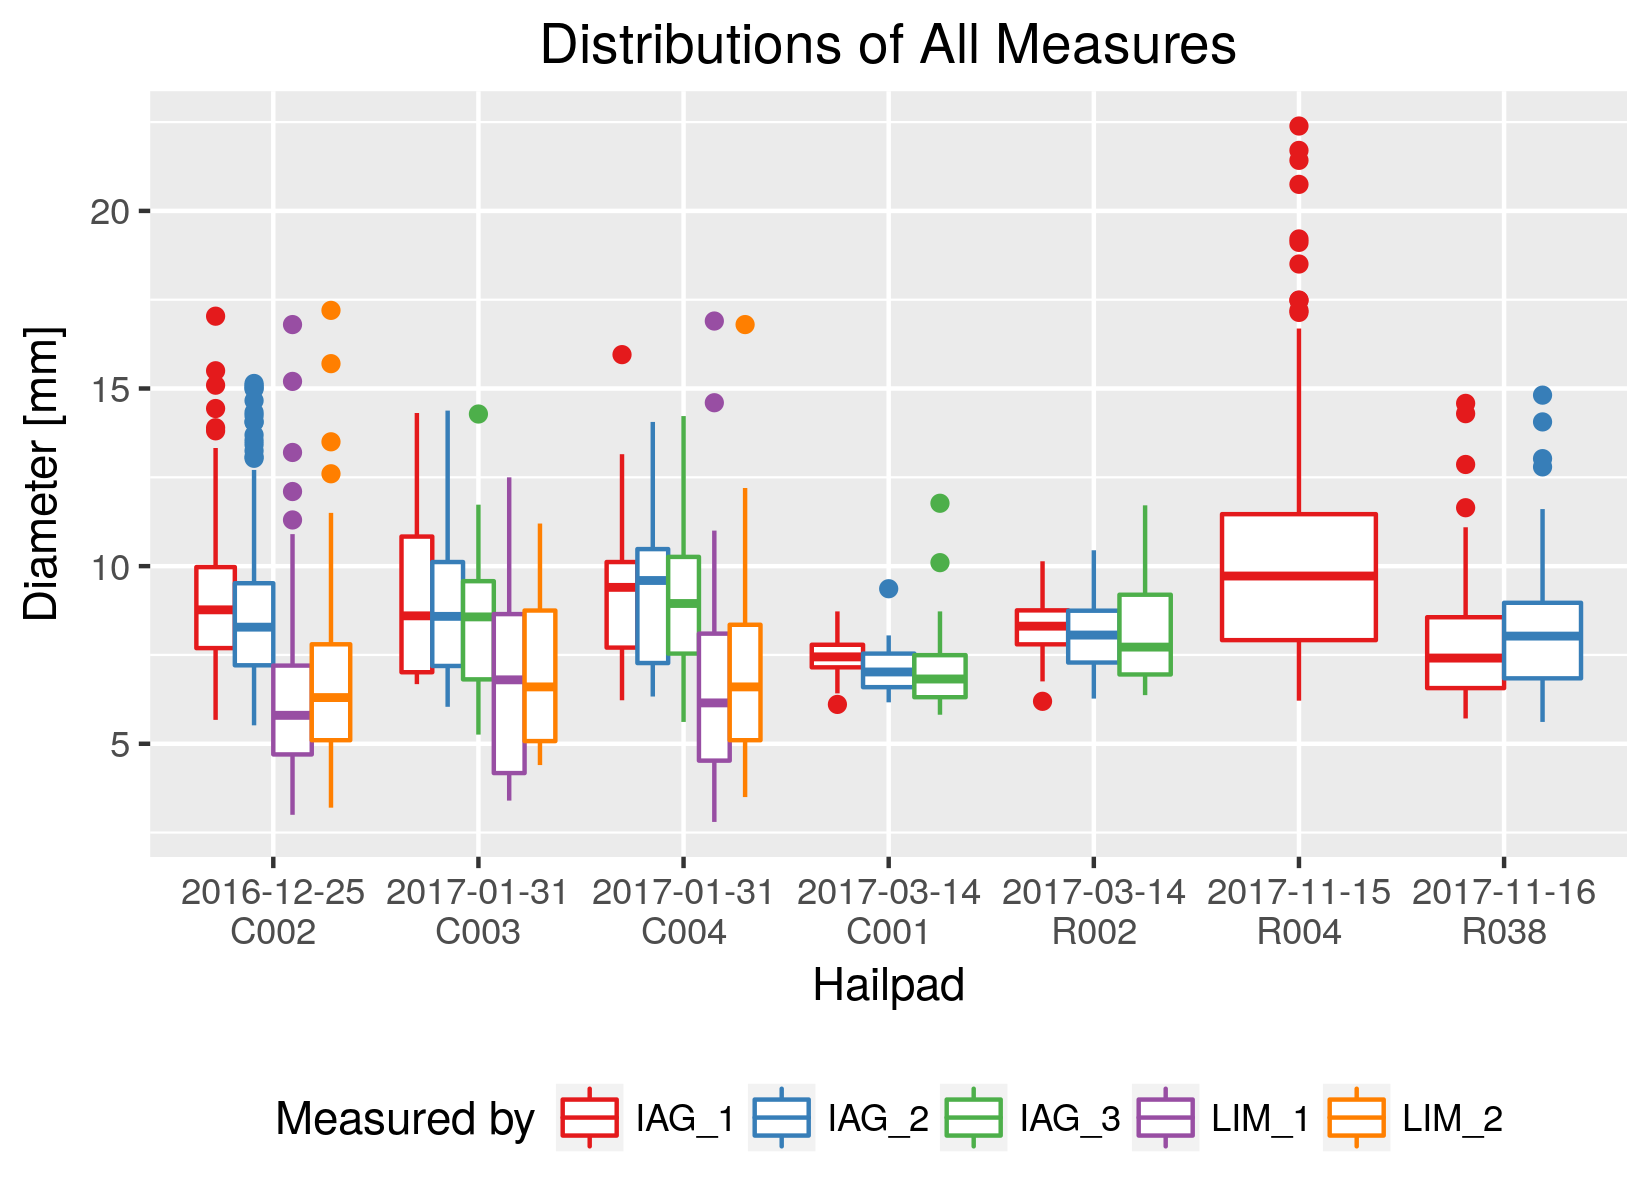
\includegraphics[width=\columnwidth]{../Hailpads_Processing/figures/measures_distribution.png}
		\legend{Fonte: Produzido pela autora.}
	\end{center}
\end{figure}

Para os casos com medidas dos dois grupos (2016-12-25 e 2017-01-31), o IAG tende a medir diâmetros maiores que o LIM, que mede mais valores extremos principalmente no caso de 2016-12-25 (os diâmetros máximos de IAG 1, LIM 1 e LIM 2 são aproximadamente iguais). Já comparando as placas para um mesmo caso (2017-01-31 e 2017-03-14), as distribuições entre o primeiro e terceiro quartil são similares, o que indica que o sistema convectivo que gerou a queda de granizo em um ponto não sofreu mudanças significativas quando gerou a queda de granizo no outro ponto. 

A \autoref{intensidade_anelfatorro} mostra a energia cinética de cada hailpad em função do diâmetro do granizo para as escalas ANELFA e TORRO. As barras de erros mais largas em relação ao diâmetro são causadas pelo desvio-padrão maior em distribuições com maiores diferenças entre cada medida (\autoref{distribuicao_tamanho}). As duas escalas mostram resultados similares entre si, com a maioria das placas relacionadas a casos minimamente intensos porém defasados em relação aos índices mínimos: os diâmetros (máximos ou típicos) são equivalentes a um índice acima da energia cinética correspondente. Isso pode estar relacionado à \autoref{mezeix}, derivada a partir de medições de tempestades na Europa, assim com às próprias escalas que também foram estabelecidas a partir de tempestades no continente europeu: condições locais e sinóticas dessa região são distintas das condições da região de estudo, principalmente comparando sistemas de latitudes médias com tropicais, fatores importantes na formação de granizo.

\begin{figure}[hbt]
	\begin{center}
		\caption{Energia cinética do hailpad em função do diâmetro do granizo considerando as escalas ANELFA e TORRO, com os índices de A0 a A2 e de H0 a H2 (\autoref{tabela_escalas}) indicados} 
		\label{intensidade_anelfatorro}
		%		\setcaptionmargin{1cm}
		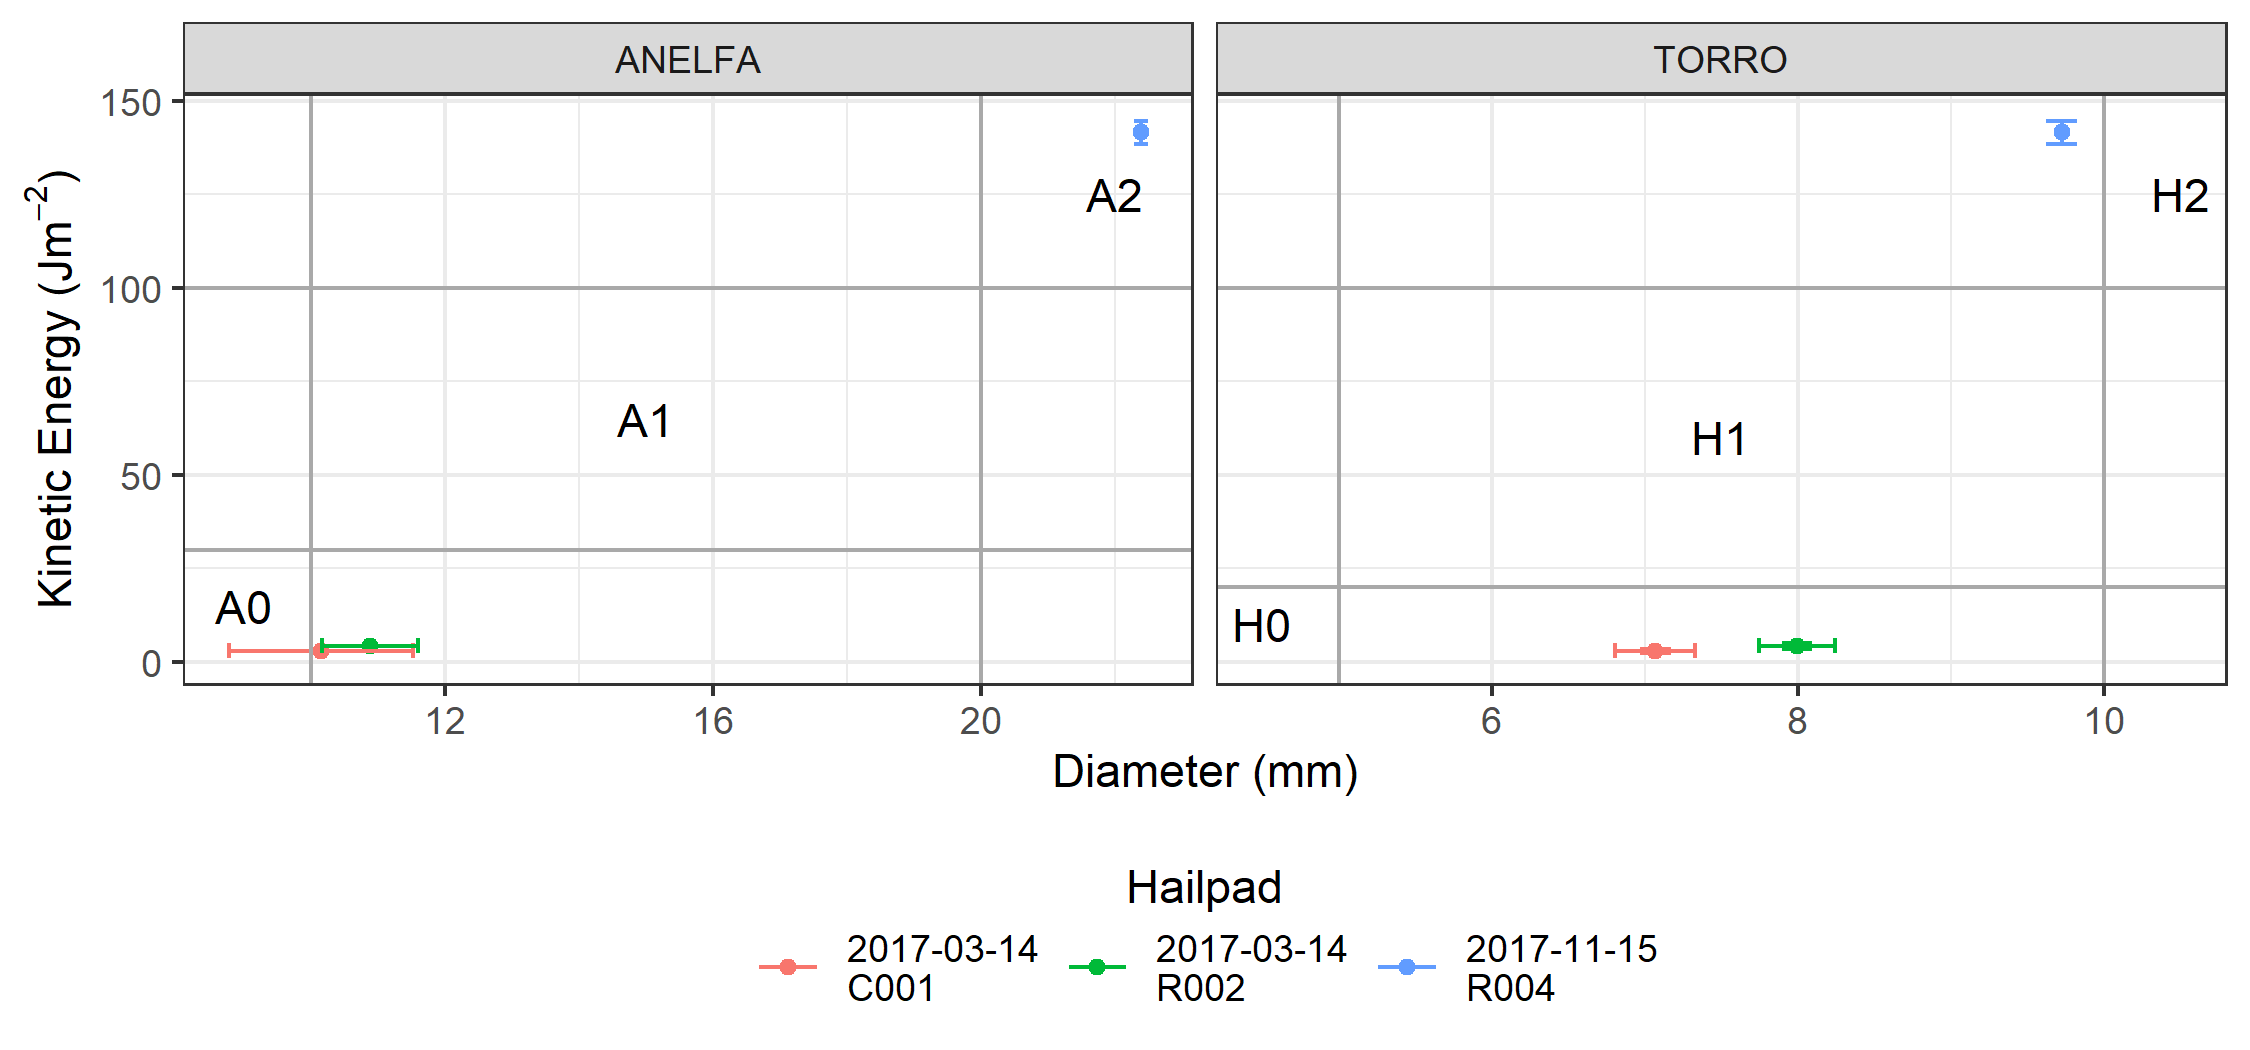
\includegraphics[width=\columnwidth]{../Hailpads_Processing/figures/data_anelfa_torro.png}
		\legend{Fonte: Produzido pela autora.}
		\nota{A escala ANELFA leva em conta o diâmetro máximo medido no hailpad, enquanto que a escala TORRO leva em conta o diâmetro típico da distribuição medida no hailpad.}
	\end{center}
\end{figure}

Dentro da escala ANELFA (painel esquerdo da \autoref{intensidade_anelfatorro}), o caso de 2017-11-15 foi considerado o mais intenso, dentro do índice A2 (danos sérios a vegetais e árvores - foram reportados danos à plantações próximas da localização do hailpad em Indaiaituba), com o caso de 2016-12-25 sendo o segundo mais intenso, dentro do índice A1 (danos à vinhas e pomares). No caso de 2017-03-14, com mais de um hailpad, a queda de granizo em Indaiatuba (placa R002) foi ligeiramente mais intensa do que em Cosmópolis (placa C004). Dentro da escala TORRO (painel direito da \autoref{intensidade_anelfatorro}) os resultados foram similares, com o case de 2017-11-15 sendo o mais intenso também mas ligeiramente fora do índice H2 (tempestade significante) e o caso de 2016-12-25 sendo o segundo mais intenso, dentro do índice H1 (tempestade potencialmente prejudicial). A queda de granizo em Indaiatuba no caso de 2017-03-14 também foi ligeiramente mais intensa do que em Cosmópolis.

A \autoref{painel_ciclo} mostra a evolução temporal da refletidade máxima (a), tamanho do sistema convectivo (b) e taxa de raios (c), enquanto que a \autoref{tabela_resumo_casos} mostra um panorama geral das características físicas relacionadas ao ciclo de vida dos casos em análise. De forma geral, a queda de granizo ocorreu dentro da fase de maturação dos sistemas convectivos, com refletividade alta, área em relativo crescimento e intensa atividade elétrica. O caso de 2017-01-31 foi o com menor tempo de vida ($0,5\:h$), área máxima ($69\:km^2$) e quantidade de raios ($8\:flashes$), mas não teve o menor tamanho de granizo: o caso de 2016-12-25 teve o menor granizo médio, enquanto que o caso de 2017-03-14 teve o menor granizo máximo (e granizo médio ligeiramente maior). O caso de 2017-03-14, por outro lado, foi o com maior tempo de vida ($6,2\:h$), refletividade máxima ($69,7\:dBZ$) e quantidade e taxa máxima de raios (15131 (4185) $flashes$ IC (CG), com taxa máxima de 125 (33) $flashes\:min^{-1}$ IC (CG)). Outro caso a ser destacado é o de 2017-11-15, com tempo de vida curto ($2,2\:h$), área máxima pequena ($253\:m^2$) e pouca quantidade de raios (menos de 200 $flashes$ somando IC e CG, taxa máxima abaixo de $10\:flashes\:min^{-1}$), mas que mostrou granizos acima de $10\:mm$ em média e granizo máximo de $22,4\:mm$. Considerando o papel do granizo na formação de raios (\autoref{teoria}), é de se esperar uma relação direta entre mudança da atividade elétrica e queda de granizo (\autoref{painel_ciclo}c), porém ela não foi consistente em todos os casos: em 2016-12-25, 2017-03-14 e 2017-11-15 há um ligeiro aumento da atividade elétrica (principalmente raios IC) até 30 minutos antes da queda de granizo, enquanto que em 2017-01-31 não há raios suficientes para determinar aumento ou diminuição da atividade elétrica, e em 2017-11-16 há um aumento da atividade elétrica depois da queda de granizo.

\begin{figure}[hbt]
	\begin{center}
		\caption{Evolução temporal da refletividade máxima em $3\:km$ (a), tamanho do sistema (b) e taxa de flashes CG e IC (c). As linhas pontilhadas indicam o momento aproximado em que houve a queda de granizo medida no hailpad} 
		\label{painel_ciclo}
		%		\setcaptionmargin{1cm}
		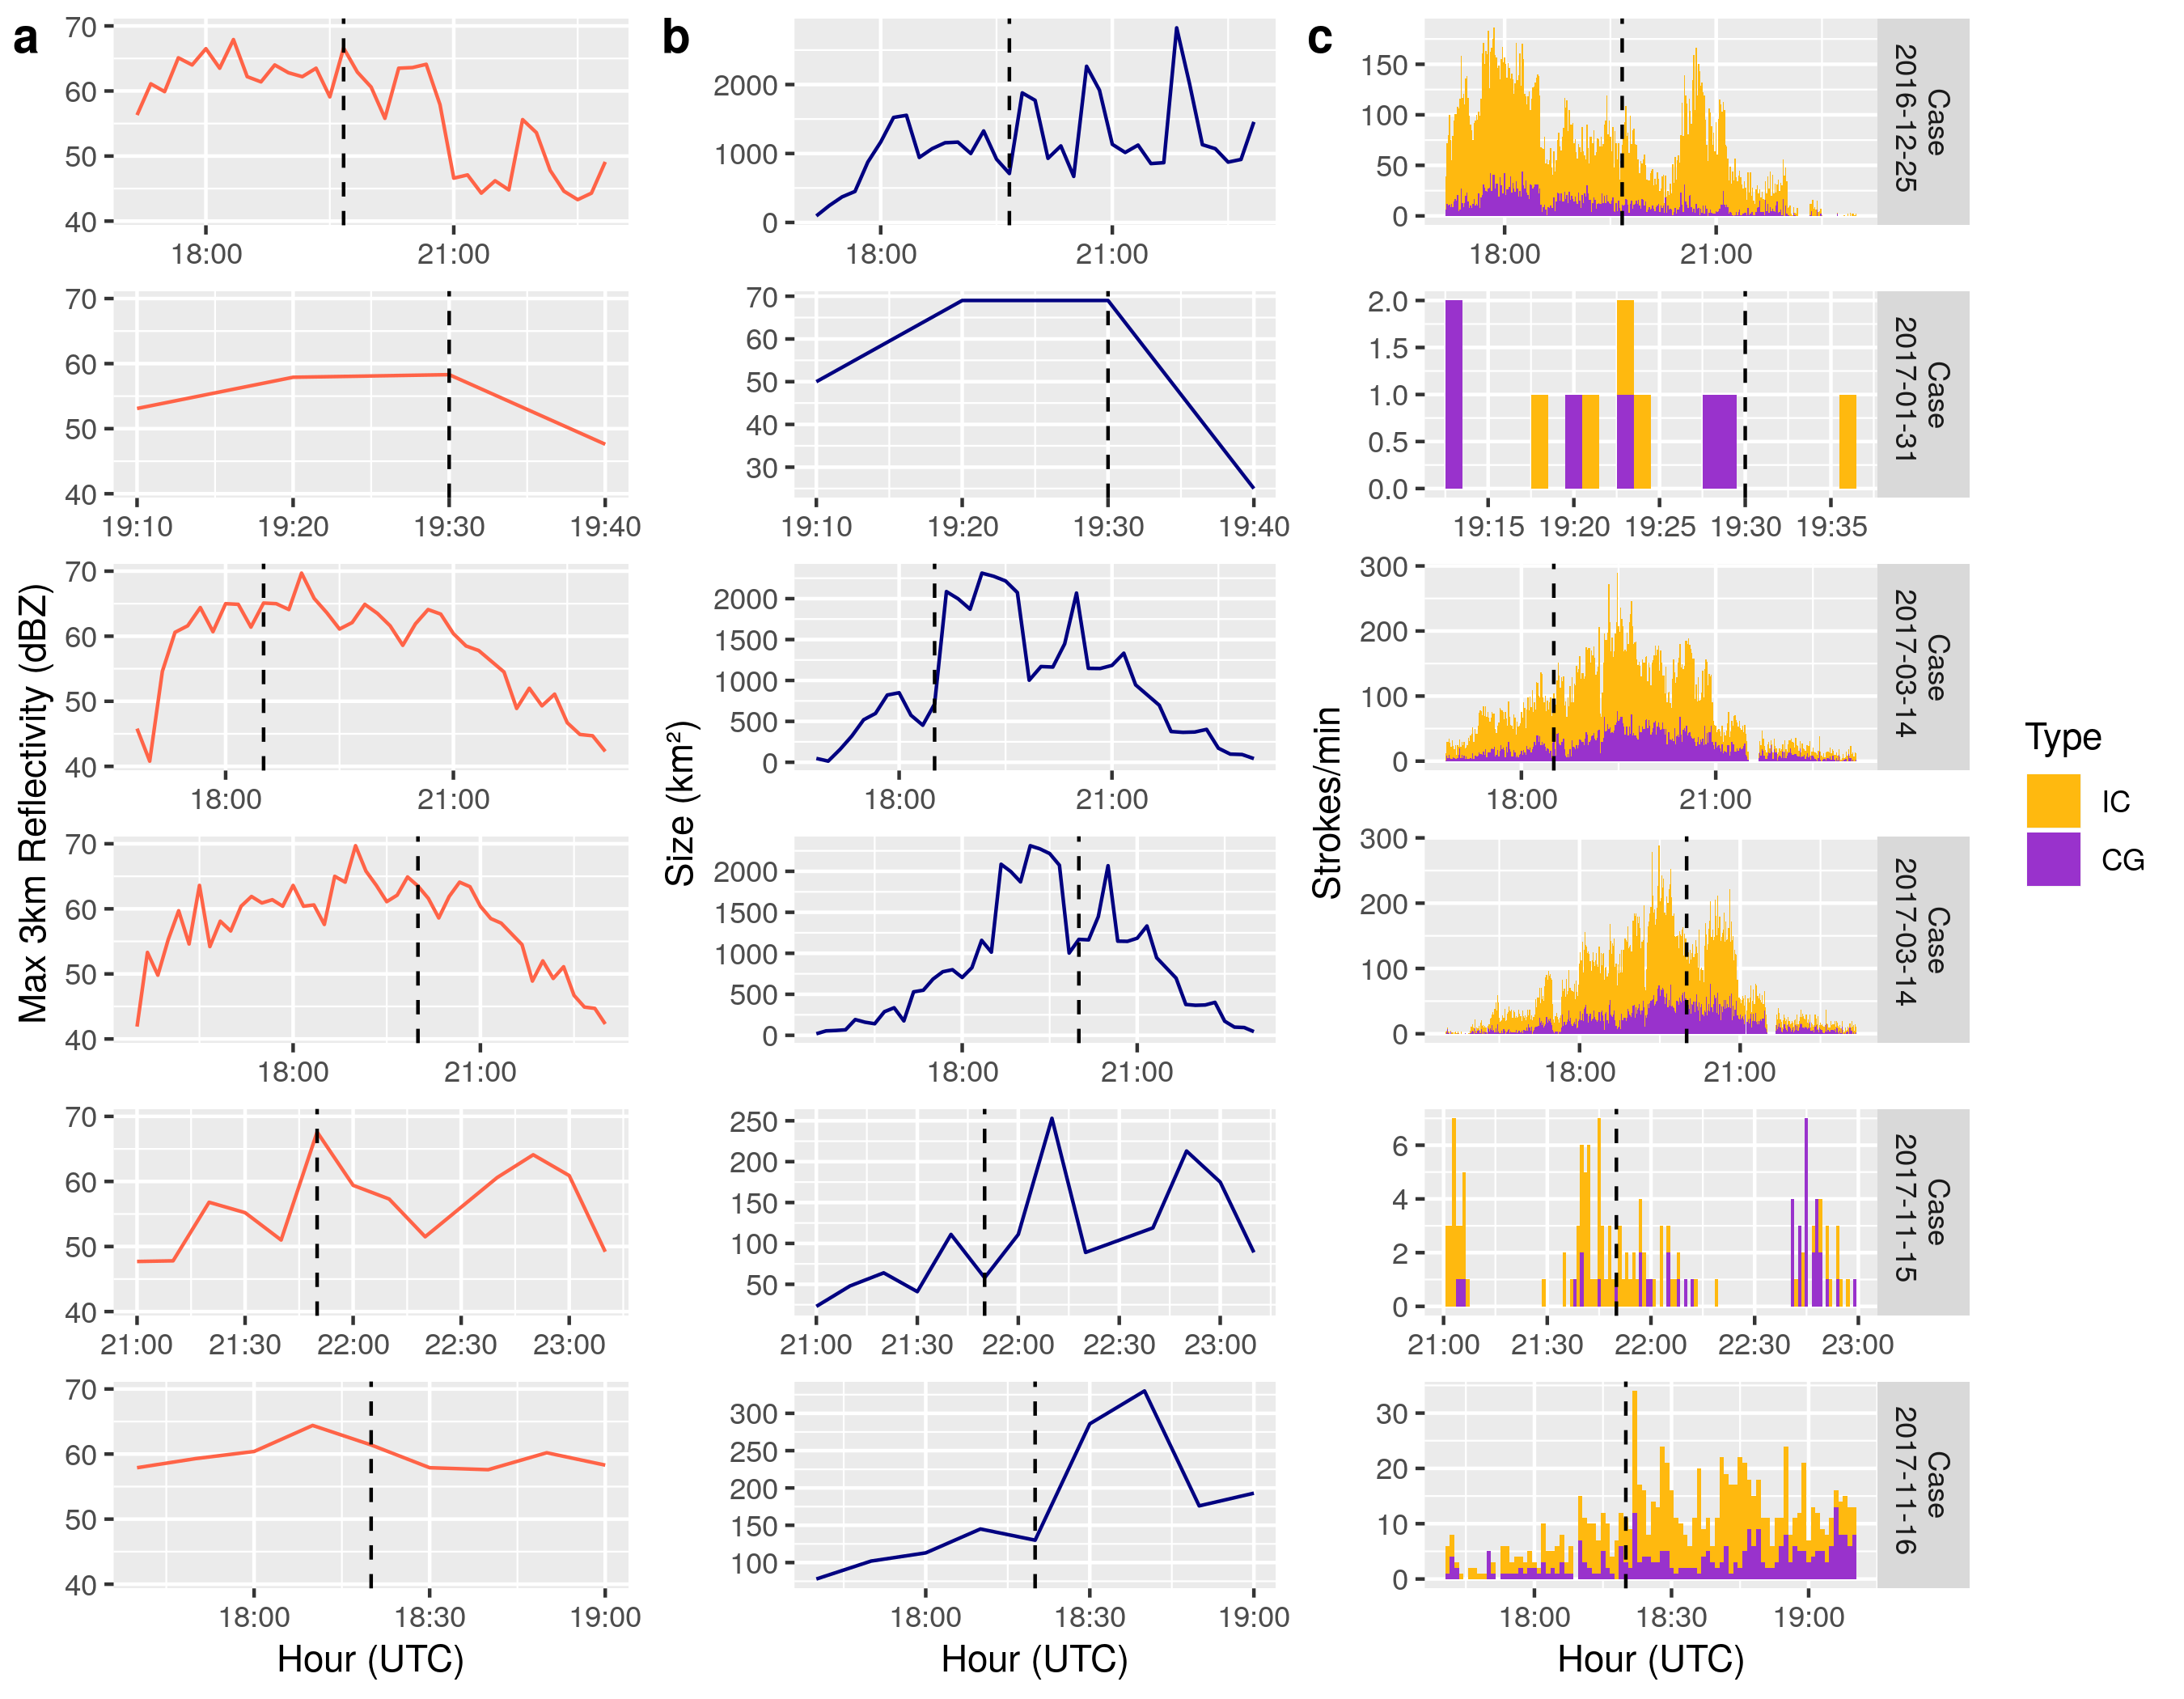
\includegraphics[width=\columnwidth]{../General_Processing/figures/cases_dbz_size_lightning.png}
		\legend{Fonte: Produzido pela autora.}
	\end{center}
\end{figure}

\begin{table}[htb]
	\IBGEtab{%
		\caption{Resumo das principais características físicas e elétricas dos casos analisados}%
		\label{tabela_resumo_casos}
	}{%
		\begin{tabularx}{\textwidth}{cY>{\hsize=1.5\hsize}Y>{\hsize=1.5\hsize}Y>{\hsize=1.5\hsize}Y>{\hsize=1.5\hsize}Y>{\hsize=0.75\hsize}Y>{\hsize=0.75\hsize}YYY}
			\toprule
			Caso & Tempo de Vida ($h$) & Z Máximo em $3\:km$ ($dBZ$) & Área Máxima ($km^2$) & Granizo Médio ($mm$) & Granizo Máximo ($mm$) & \multicolumn{2}{>{\hsize=2\hsize}Y}{Total de Raios ($flashes$)} & \multicolumn{2}{>{\hsize=2\hsize}Y}{Taxa Máxima de Raios ($flashes\ min^{-1}$)} \\
			\cmidrule(l){7-10}
			 & & & & & & IC & CG & IC & CG \\
			\midrule
			2016-12-25 & $5,7$ & $67,9$ & $2822$ & $7,6$ & $17,2$ & $13130$ & $2260$ & $104$ & $26$ \\
			\midrule 
			2017-01-31 & $0,5$ & $58,3$ & $69$ & $8,2$ & $16,9$ & $4$ & $4$ & $1$ & $1$ \\
			\midrule 
			2017-03-14 & $6,2$ & $69,7$ & $2312$ & $7,8$ & $11,8$ & $15131$ & $4185$ & $125$ & $33$ \\
			\midrule 
			2017-11-15 & $2,2$ & $67,6$ & $253$ & $10,3$ & $22,4$ & $86$ & $29$ & $8$ & $3$ \\
			\midrule 
			2017-11-16 & $1,3$ & $64,4$ & $330$ & $8$ & $14,8$ & $528$ & $227$ & $19$ & $8$ \\
			\bottomrule
		\end{tabularx}%
	}{%
		\fonte{Produzido pela autora.}%
	}
\end{table}


A partir dos resultados descritos nesta seção, dois casos foram escolhidos para uma análise mais detalhada:

\begin{alineas}
	\item \textbf{2017-03-14}: Classificado como tempestade com queda de granizo de baixa intensidade, este caso teve alta atividade elétrica durante seu longo ciclo de vida, gerando queda de granizo em dois pontos diferentes. Os dois momentos em que houve queda de granizo serão comparados em relação à estrutura e cinemática da nuvem;
	\item \textbf{2017-11-15}: Classificado com tempestade com queda de granizo de intensidade significativa, este caso teve baixa atividade elétrica, o que não é esperado em uma tempestade com produção de granizo suficiente para cair no solo com tamanho considerável. A microfísica e cinemática desta tempestade com ciclo de vida mais curto ajudará a explicar esse comportamento.
\end{alineas}

\section{Estudos de Caso}\label{estudo_casos}

\subsection{2017-03-14}

\subsubsection{Ambiente Sinótico}\label{sinotica_201703014}

A influência de uma frente fria no litoral de São Paulo e do Rio de Janeiro durante a madrugada foi determinante para o disparo de sistemas convectivos no estado de São Paulo durante a tarde. O sistema frontal em si se deslocou para o Oceano Atlântico ao longo do dia - às 1200 UTC (Figura\autoref{era5_2017031412_jets}), o sistema está à leste de $30^{\circ}W$ - mas favoreceu a convergência de umidade na região de estudo (não mostrado). Às 1200 UTC, a radissondagem (\autoref{sondagem_20170314}) mostra uma camada úmida entre a superfície e $600\:hPa$, mas com CAPE (\textit{Convective Available Potential Energy}, Energia Potencial Disponível para Convecção) nulo e pouco cisalhamento (mesma condição no resto do estado, como mostra a Figura\autoref{era5_2017031412_cape}). Já às 1500 UTC (Figura\autoref{era5_2017031415_cape}), o potencial para convecção (CAPE entre 500 e $1500\:J\:kg^{-1}$) e o cisalhamento (de até 10 nós) aumentaram, disparando sistemas convectivos no centro do estado de São Paulo. A \autoref{goes16_sp_20170314} mostra a propagação e intensificação de sistemas convectivos na região de estudo aproximadamente às 1800 (a) e 2000 UTC (b).

\begin{figure}[htb]
	\begin{center}
		\caption{Campos da reanálise do ERA5 em 2017-03-14: Pressão ao nível médio do mar, espessura entre $1000$ e $500\:hPa$ e velocidade do vento em $250\:hPa$ às 1200 UTC (a); altura geopotencial em $850\:hPa$, cisalhamento do vento entre $1000$ e $500\:hPa$ e CAPE em superfície às 1200 (b) e 1500 UTC, no domínio do Estado de São Paulo (c)} 
		\label{era5_20170314_main}
		\subfloat[]{\includegraphics[width=0.5\columnwidth]{../Reanalysis_Processing/figures/ERA5_SA_sfc-jets_201703141200.png}
			\label{era5_2017031412_jets}}
		\subfloat[]{\includegraphics[width=0.5\columnwidth]{../Reanalysis_Processing/figures/ERA5_SA_cape-shear_2017031412.png}
			\label{era5_2017031412_cape}} \\
		\subfloat[]{\includegraphics[width=0.5\columnwidth]{../Reanalysis_Processing/figures/ERA5_SP-BR_cape-shear_2017031415.png}
			\label{era5_2017031415_cape}} \\
		\legend{Fonte: Produzido pela autora.}
	\end{center}
\end{figure}

\begin{figure}[hp]
	\begin{center}
		\caption{Plotagem Skew-T Log-P da radiossondagem do Campo de Marte (SP) com hodógrafa do vento e índices CAPE e CIN em 2017-03-14 1200 UTC.} 
		\label{sondagem_20170314}
		%		\setcaptionmargin{1cm}
		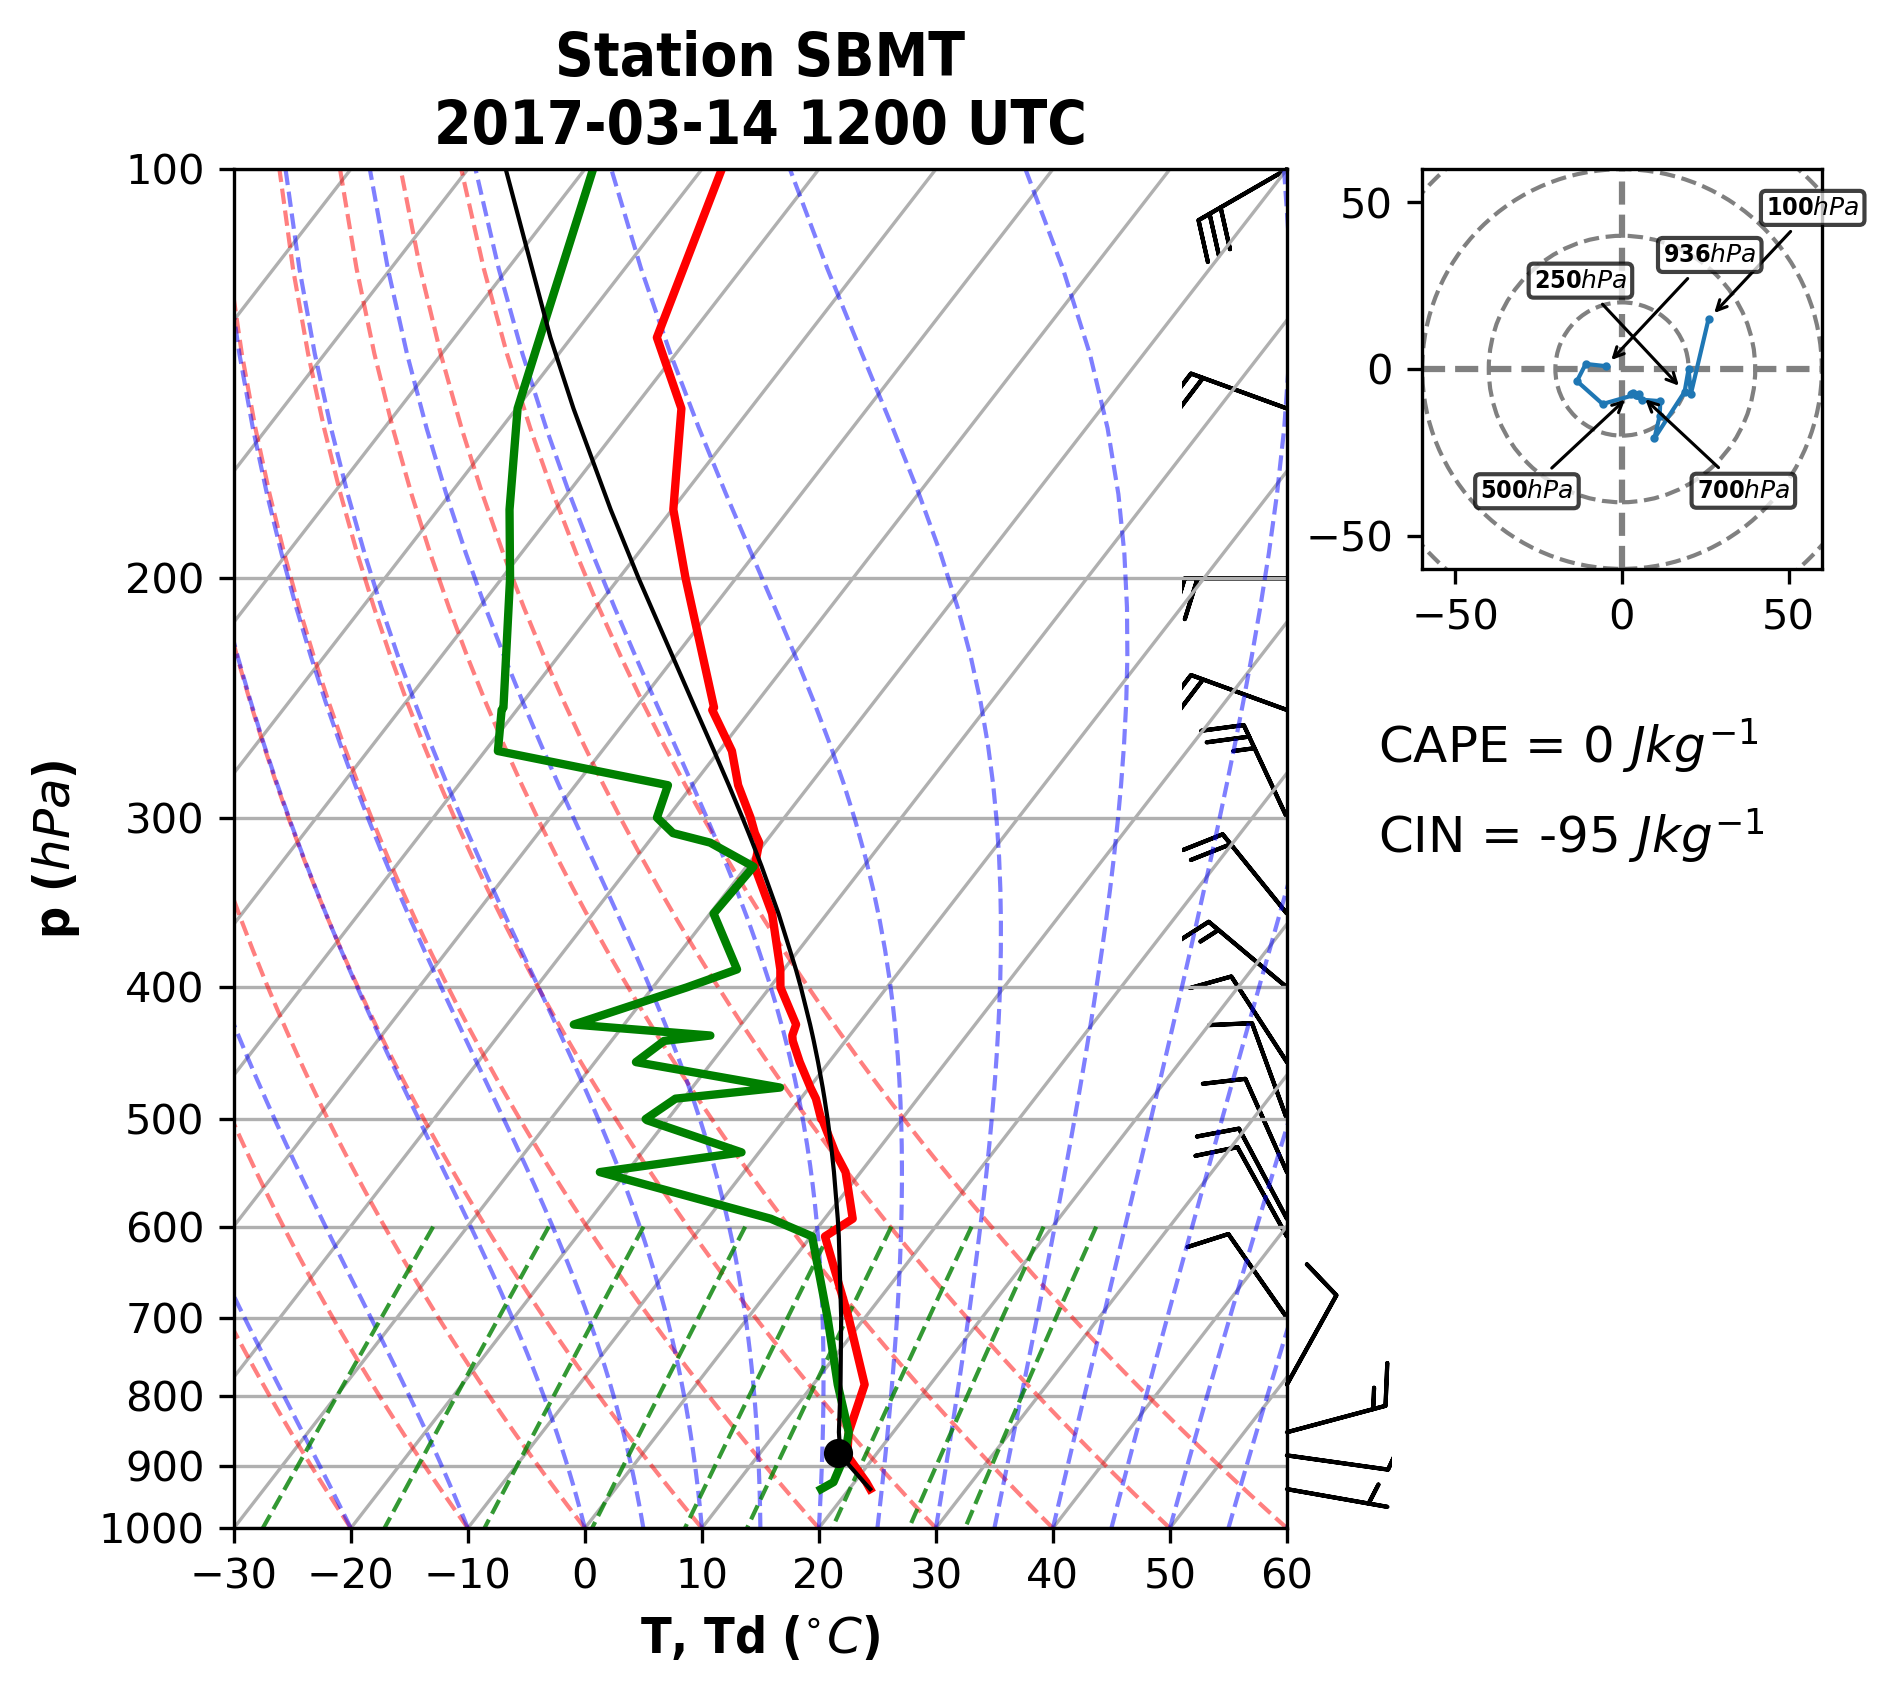
\includegraphics[width=0.75\columnwidth]{../Sounding_Processing/figures/sounding_SBMT2017031412UTC.png}
		\legend{Fonte: Produzido pela autora.}
	\end{center}
\end{figure}

%\begin{figure}[htb]
%	\begin{center}
%		\caption{Imagem de satélite do canal 13 do GOES-16 mostrando a temperatura de brilho do topo das nuvens na América do Sul em 2017-03-14 1751 UTC.} 
%		\label{goes16_sa_20170314}
%		%		\setcaptionmargin{1cm}
%		\includegraphics[width=0.75\columnwidth]{../Satellite_Processing/figures/Band_13/GOES16_B13_SA_SD201703141751.png}
%		\legend{Fonte: Produzido pela autora.}
%	\end{center}
%\end{figure}
%
\begin{figure}[hp]
	\begin{center}
		\caption{Imagem de satélite do canal 13 do GOES-16 mostrando a temperatura de brilho do topo das nuvens no estado de São Paulo em 2017-03-14 1751 (a) e 1951 UTC (b).} 
		\label{goes16_sp_20170314}
		\subfloat[]{\includegraphics[width=0.5\columnwidth]{../Satellite_Processing/figures/Band_13/GOES16_B13_SP-BR_SD201703141751.png}
			\label{goes16_sp_20170314_1}}
		\subfloat[]{\includegraphics[width=0.5\columnwidth]{../Satellite_Processing/figures/Band_13/GOES16_B13_SP-BR_SD201703141951.png}
			\label{goes16_sp_20170314_2}} \\
		\legend{Fonte: Produzido pela autora.}
	\end{center}
\end{figure}

\subsubsection{Eletrificação}\label{elec_201703014}

\begin{figure}[htb]
	\begin{center}
		\caption{Rastreamento (a) e localização dos flashes IC e CG (b) do sistema convectivo responsável pelas quedas de granizo em Cosmópolis e Indaiatuba em 2017-03-14. Os triângulos pretos indicam a localização dos hailpads.} 
		\label{track_flashes_20170314}
		%		\setcaptionmargin{1cm}
		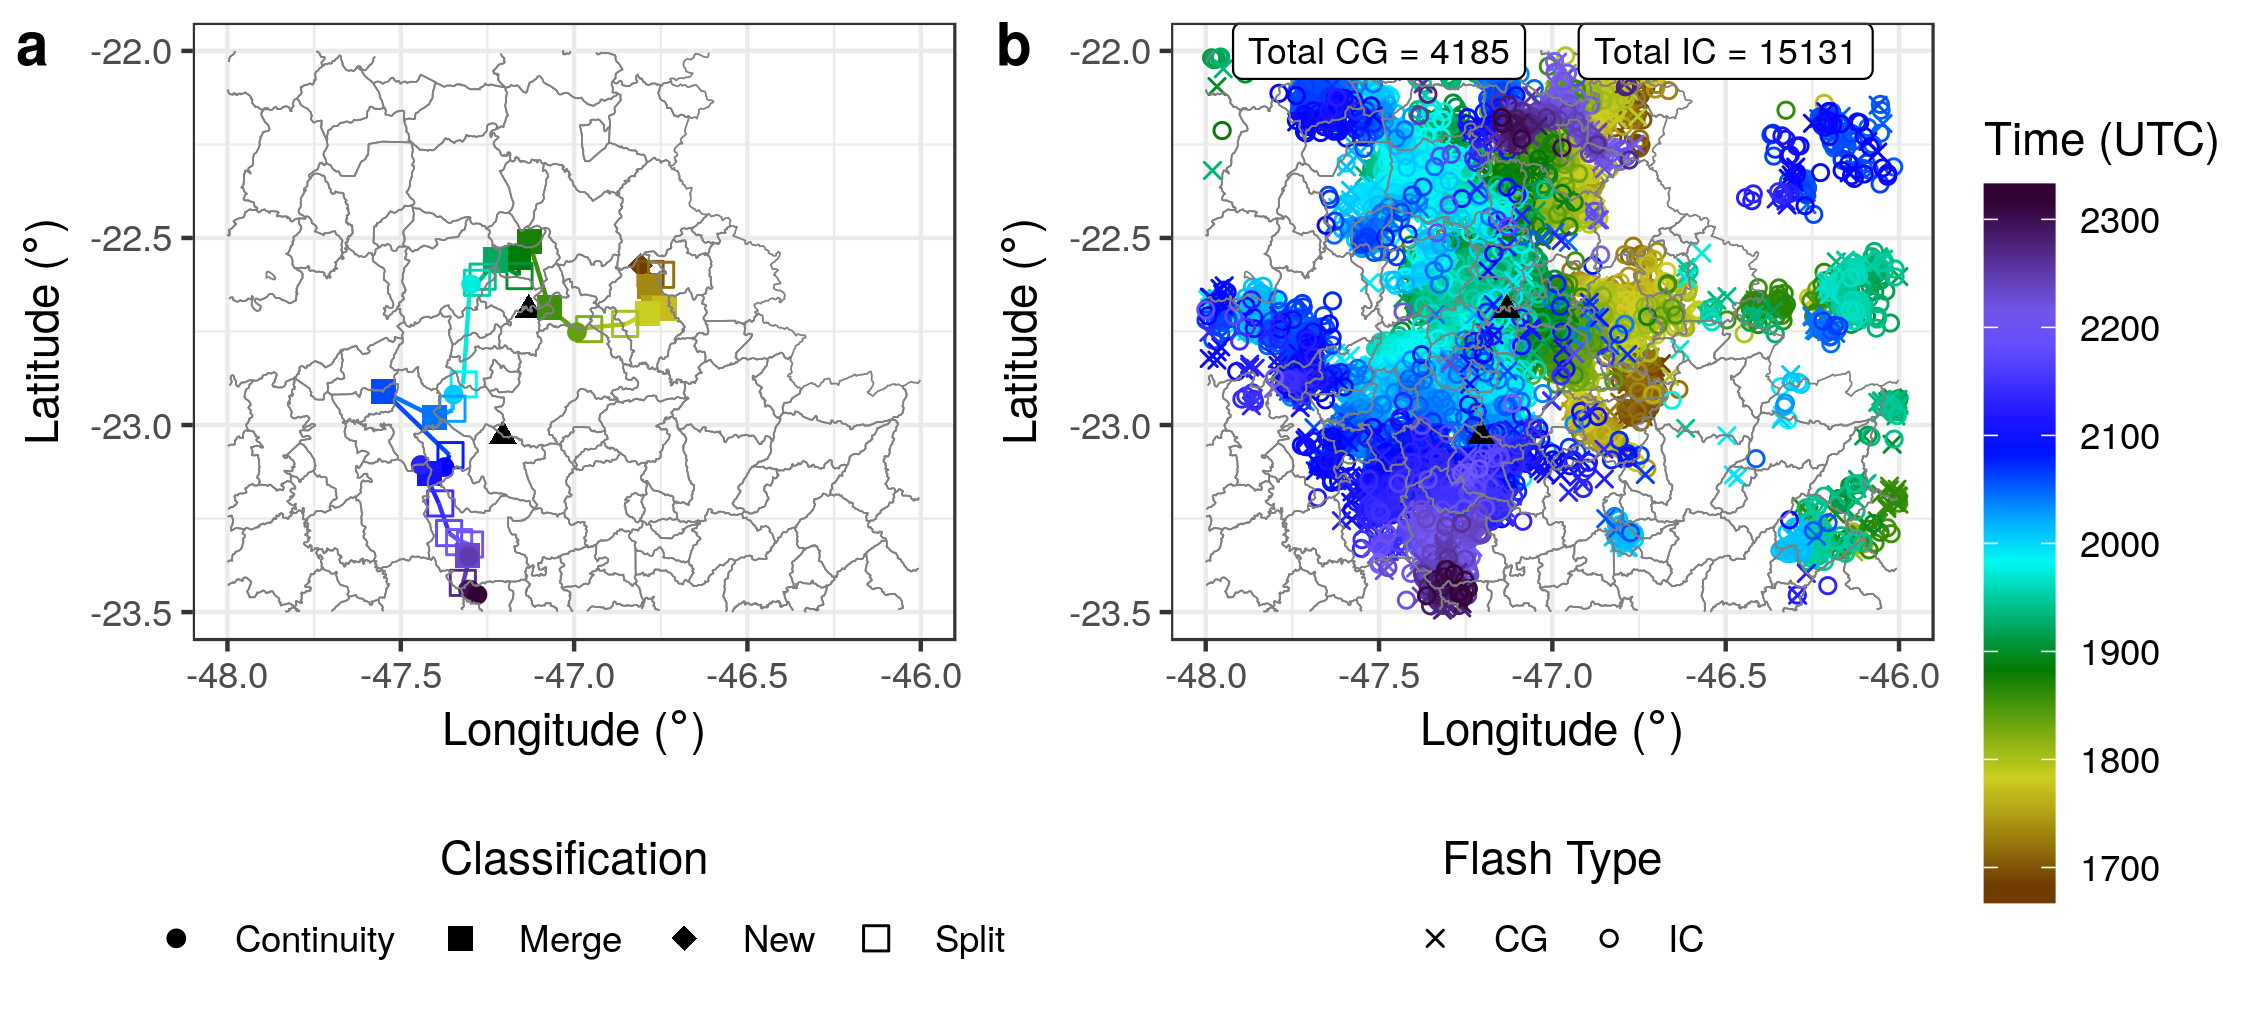
\includegraphics[width=\columnwidth]{../General_Processing/figures/track_flashes_20170314.png}
		\legend{Fonte: Produzido pela autora.}
	\end{center}
\end{figure}

\subsubsection{Microfísica}\label{micro_201703014}

\begin{figure}[hp]
	\centering
	\caption{Corte horizontal em $3\:km$ de altura e vertical entre os pontos A e B de campos do radar da FCTH em 2017-03-14 1827 UTC, quando houve queda de granizo em Cosmópolis: Refletividade corrigida (a) e diferencial (b), fase diferencial específica (c) e coeficiente de correlação (d). O 'x' indica a localização do hailpad e as isotermas de $0$ e $-40^{\circ}C$ foram definidas a partir da radiossondagem de SMBT}
	\label{radar_20170314_1}
	\vspace{-5pt}
	\includegraphics[width=\columnwidth]{../Radar_Processing/figures/ppis/classification/FCTH Corrected Reflectivity 2017-03-14 1827 UTC.png}
		\label{z_20170314_1} \\
	\vspace{-15pt}
	\includegraphics[width=\columnwidth]{../Radar_Processing/figures/ppis/classification/FCTH Differential Reflectivity 2017-03-14 1827 UTC.png}
		\label{zdr_20170314_1} \\
	\vspace{-15pt}
	\includegraphics[width=\columnwidth]{../Radar_Processing/figures/ppis/classification/FCTH Specific Differential Phase 2017-03-14 1827 UTC.png}
		\label{kdp_20170314_1} \\
	\vspace{-15pt}
	\includegraphics[width=\columnwidth]{../Radar_Processing/figures/ppis/classification/FCTH Cross Correlation Ratio 2017-03-14 1827 UTC.png}
		\label{rho_20170314_1} \\
	\vspace{-5pt}
	\legend{Fonte: Produzido pela autora.}
\end{figure}

\begin{figure}[htb]
	\centering
	\caption{Corte horizontal em $3\:km$ de altura e vertical entre os pontos A e B de campos derivados do radar da FCTH em 2017-03-14 1827 UTC, quando houve queda de granizo em Cosmópolis: Identificação de hidrometeoros (a) e massas de água líquida (b) e gelo (c). O 'x' indica a localização do hailpad e as isotermas de $0$ e $-40^{\circ}C$ foram definidas a partir da radiossondagem de SMBT} 
	\label{radar_derived_20170314_1}
	\vspace{-5pt}
	\includegraphics[width=\columnwidth]{../Radar_Processing/figures/ppis/classification/FCTH Hydrometeor ID 2017-03-14 1827 UTC.png}
		\label{hid_20170314_1} \\
	\vspace{-15pt}
	\includegraphics[width=\columnwidth]{../Radar_Processing/figures/ppis/classification/FCTH Liquid Water Mass 2017-03-14 1827 UTC.png}
		\label{ml_20170314_1} \\
	\vspace{-15pt}
	\includegraphics[width=\columnwidth]{../Radar_Processing/figures/ppis/classification/FCTH Ice Water Mass 2017-03-14 1827 UTC.png}
		\label{mi_20170314_1} \\
	\vspace{-5pt}
	\legend{Fonte: Produzido pela autora.}
\end{figure}


\begin{figure}[hp]
	\centering
	\caption{Corte horizontal em $3\:km$ de altura e vertical entre os pontos A e B de campos do radar da FCTH em 2017-03-14 1957 UTC, quando houve queda de granizo em Indaiatuba: Refletividade corrigida (a) e diferencial (b), fase diferencial específica (c) e coeficiente de correlação (d). O 'x' indica a localização do hailpad e as isotermas de $0$ e $-40^{\circ}C$ foram definidas a partir da radiossondagem de SMBT}
	\label{radar_20170314_2}
	\vspace{-5pt}
	\includegraphics[width=\columnwidth]{../Radar_Processing/figures/ppis/classification/FCTH Corrected Reflectivity 2017-03-14 1957 UTC.png}
	\label{z_20170314_2} \\
	\vspace{-15pt}
	\includegraphics[width=\columnwidth]{../Radar_Processing/figures/ppis/classification/FCTH Differential Reflectivity 2017-03-14 1957 UTC.png}
	\label{zdr_20170314_2} \\
	\vspace{-15pt}
	\includegraphics[width=\columnwidth]{../Radar_Processing/figures/ppis/classification/FCTH Specific Differential Phase 2017-03-14 1957 UTC.png}
	\label{kdp_20170314_2} \\
	\vspace{-15pt}
	\includegraphics[width=\columnwidth]{../Radar_Processing/figures/ppis/classification/FCTH Cross Correlation Ratio 2017-03-14 1957 UTC.png}
	\label{rho_20170314_2} \\
	\vspace{-5pt}
	\legend{Fonte: Produzido pela autora.}
\end{figure}

\begin{figure}[htb]
	\centering
	\caption{Corte horizontal em $3\:km$ de altura e vertical entre os pontos A e B de campos derivados do radar da FCTH em 2017-03-14 1957 UTC, quando houve queda de granizo em Indaiatuba: Identificação de hidrometeoros (a) e massas de água líquida (b) e gelo (c). O 'x' indica a localização do hailpad e as isotermas de $0$ e $-40^{\circ}C$ foram definidas a partir da radiossondagem de SMBT} 
	\label{radar_derived_20170314_2}
	\vspace{-5pt}
	\includegraphics[width=\columnwidth]{../Radar_Processing/figures/ppis/classification/FCTH Hydrometeor ID 2017-03-14 1957 UTC.png}
	\label{hid_20170314_2} \\
	\vspace{-15pt}
	\includegraphics[width=\columnwidth]{../Radar_Processing/figures/ppis/classification/FCTH Liquid Water Mass 2017-03-14 1957 UTC.png}
	\label{ml_20170314_2} \\
	\vspace{-15pt}
	\includegraphics[width=\columnwidth]{../Radar_Processing/figures/ppis/classification/FCTH Ice Water Mass 2017-03-14 1957 UTC.png}
	\label{mi_20170314_2} \\
	\vspace{-5pt}
	\legend{Fonte: Produzido pela autora.}
\end{figure}

\subsubsection{Cinemática}\label{cinematica_201703014}

\begin{figure}[htb]
	\centering
	\caption{Corte horizontal em $3\:km$ de altura e vertical entre os pontos A e B de refletividade e velocidade do vento (correntes ascendentes e descendentes máximas no painel da esquerda, escoamento no painel da direita) derivado por Multi-Doppler em 2017-03-14 às 1820 (a) e 1830 UTC (b), quando houve queda de granizo em Cosmópolis. O 'x' indica a localização do hailpad e as isotermas de $0$ e $-40^{\circ}C$ foram definidas a partir da radiossondagem de SMBT} 
	\label{doppler_20170314_1}
	\vspace{-5pt}
	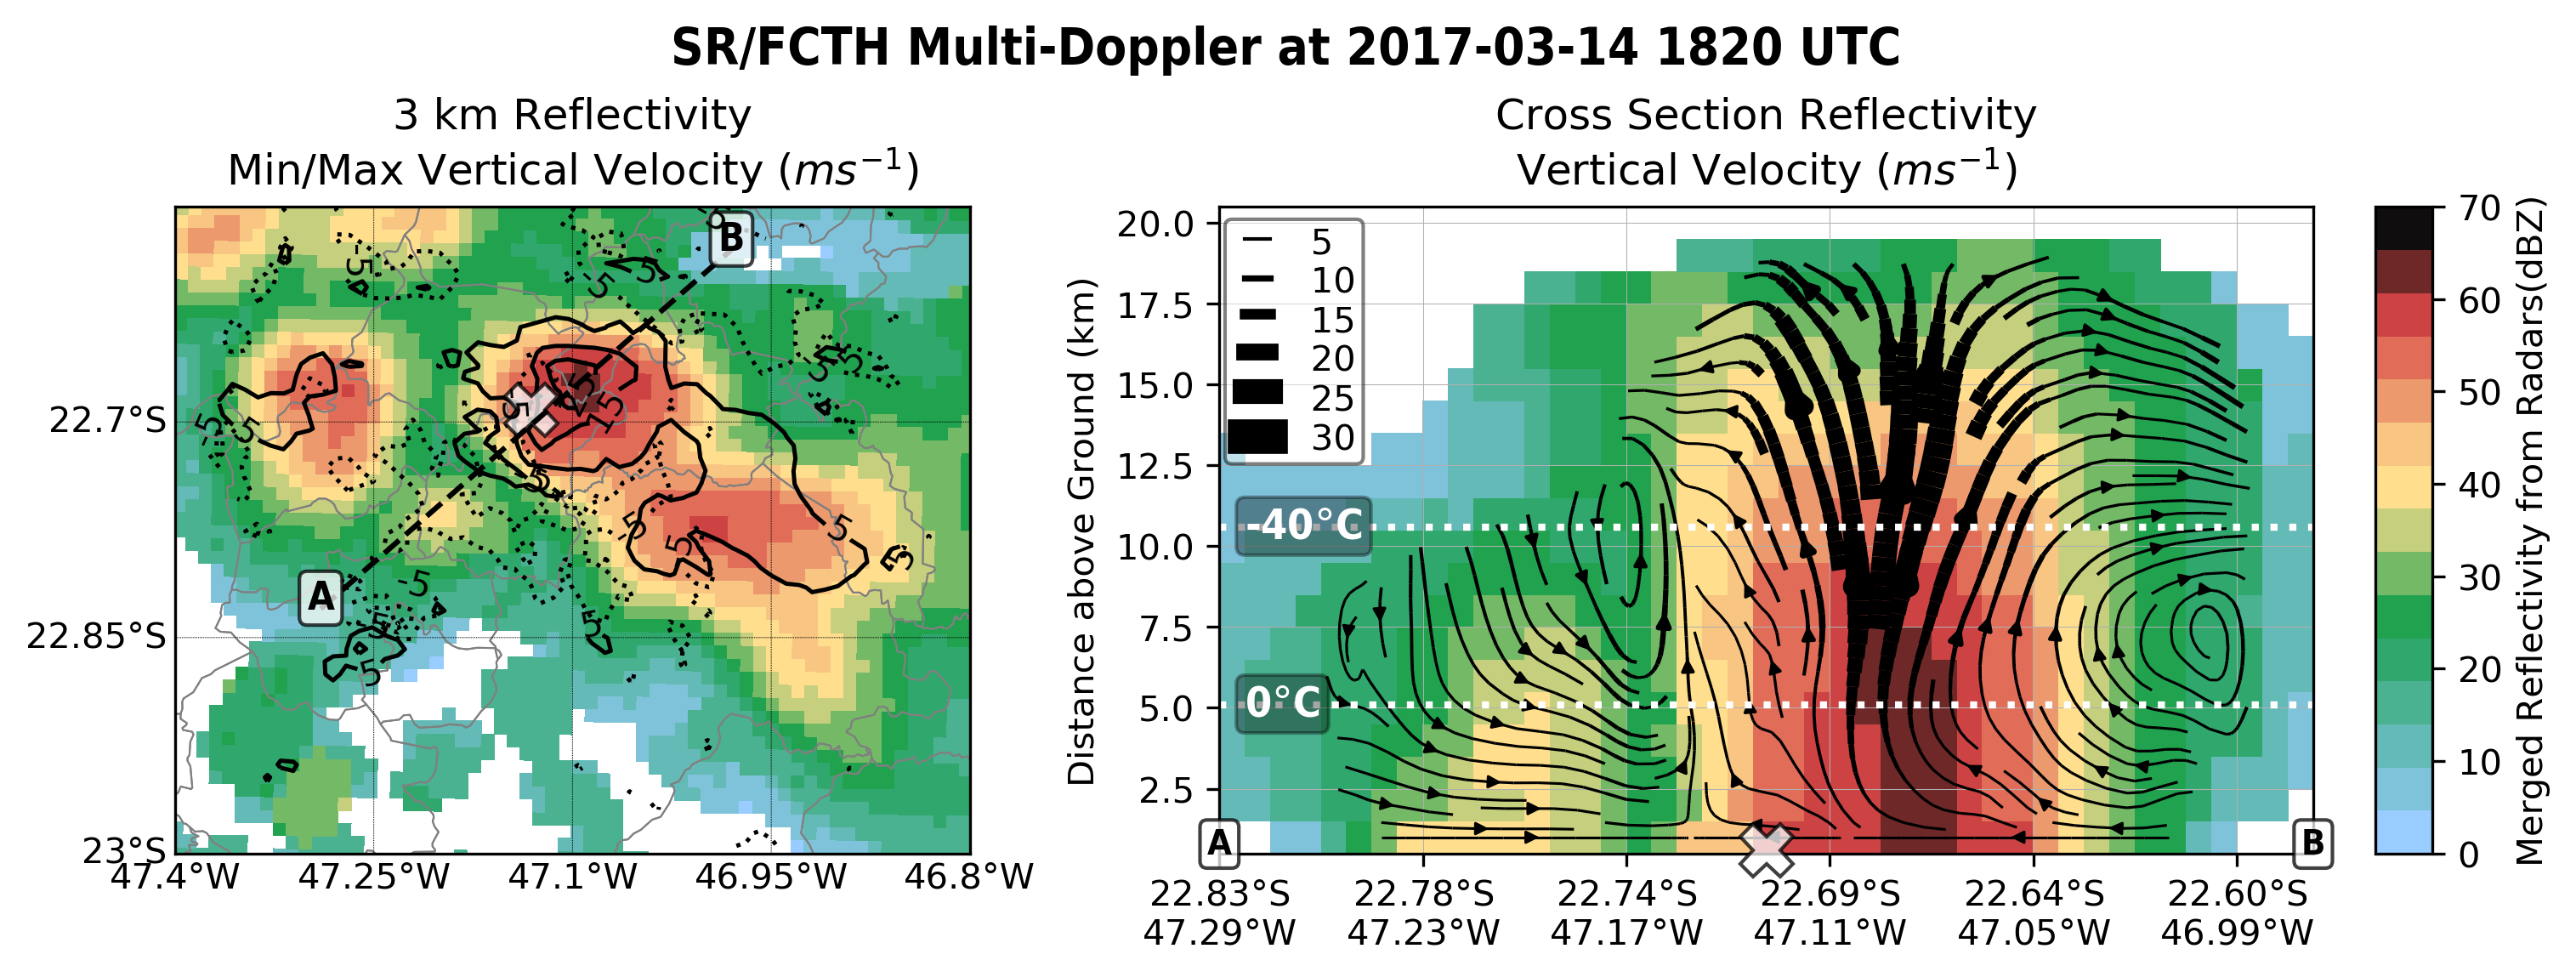
\includegraphics[width=\columnwidth]{../MultiDoppler_Processing/figures/SR-FCTH 2017-03-14 1820 UTC.png}
		\label{dopplera_20170314_1} \\
	\vspace{-15pt}
	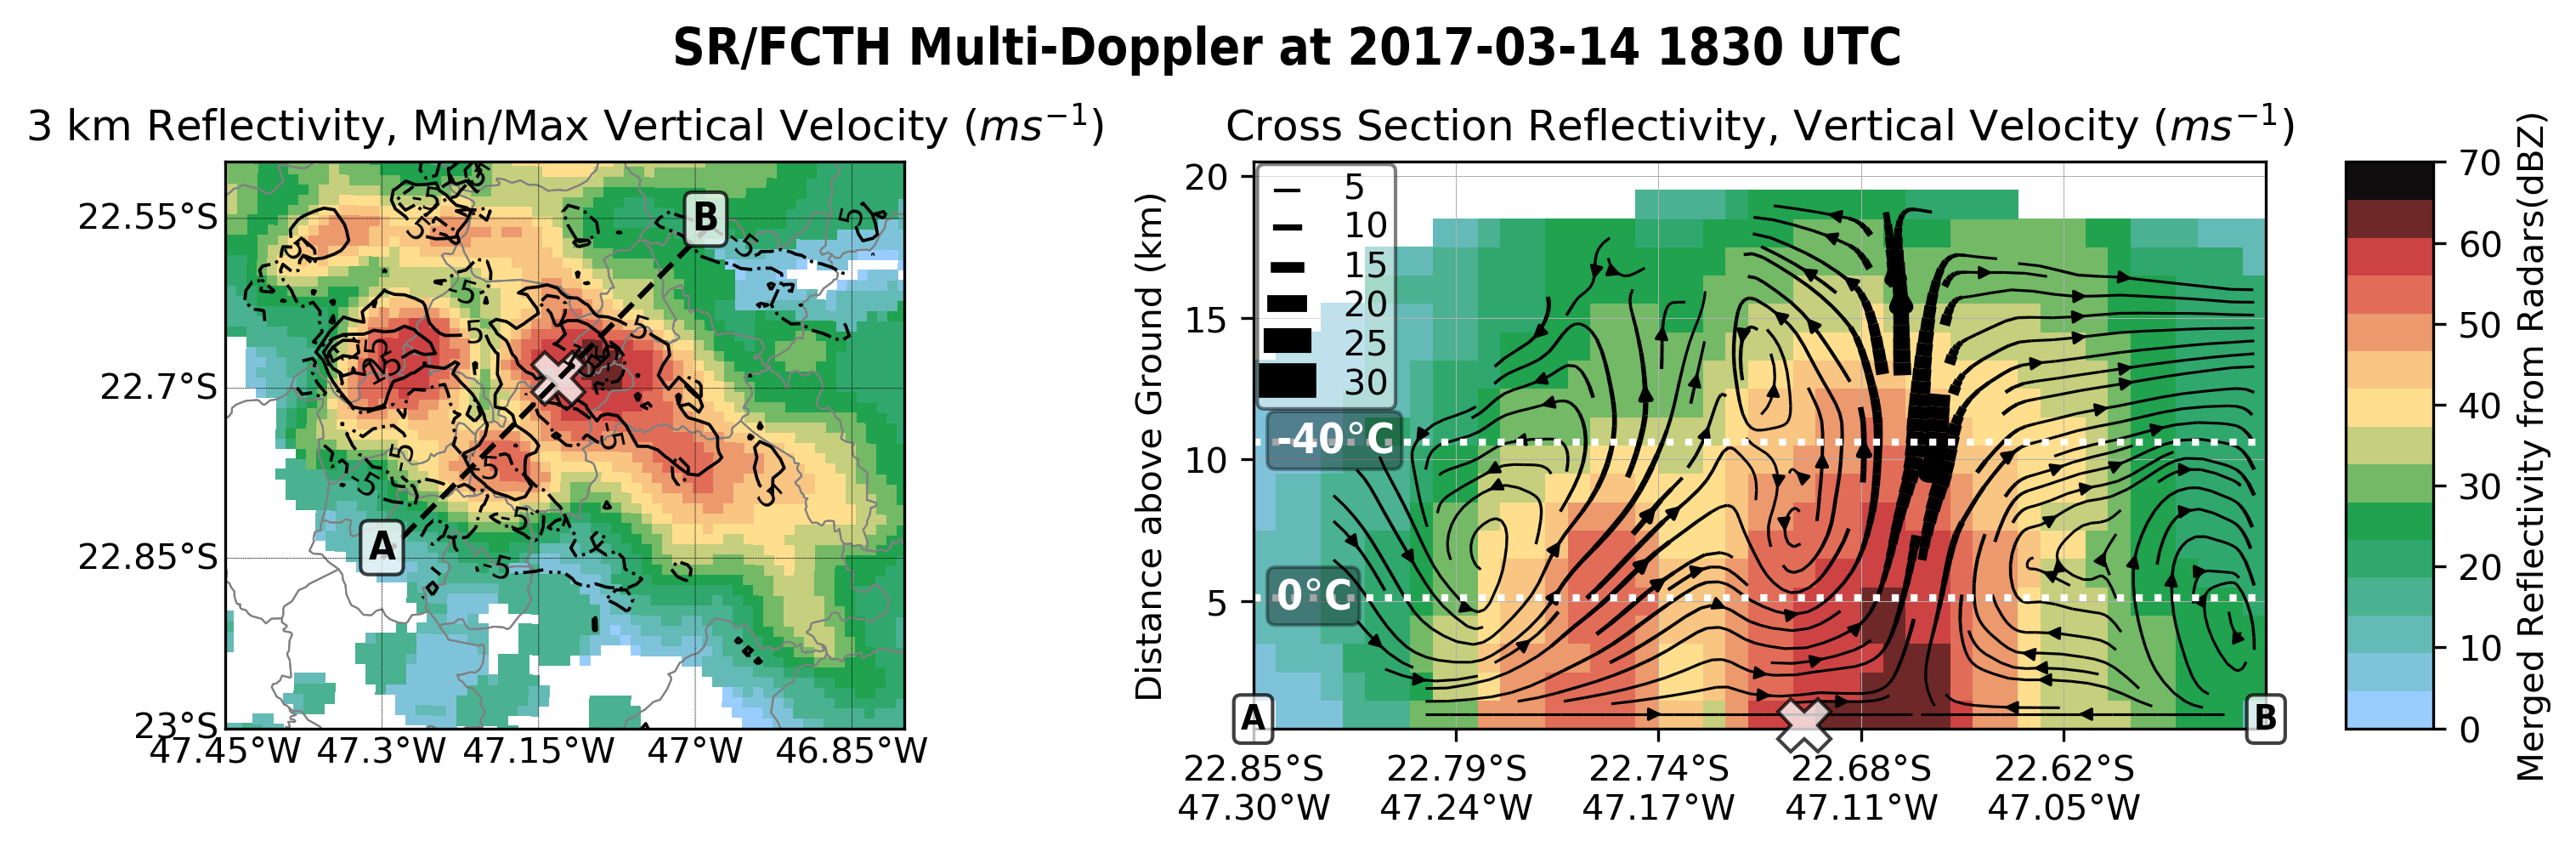
\includegraphics[width=\columnwidth]{../MultiDoppler_Processing/figures/SR-FCTH 2017-03-14 1830 UTC.png}
		\label{dopplerb_20170314_1} \\
	\vspace{-5pt}
	\legend{Fonte: Produzido pela autora.}
\end{figure}

\begin{figure}[htb]
	\centering
	\caption{Corte horizontal em $3\:km$ de altura e vertical entre os pontos A e B de refletividade e velocidade do vento (correntes ascendentes e descendentes máximas no painel da esquerda, escoamento no painel da direita) derivado por Multi-Doppler em 2017-03-14 às 1950 (a) e 2000 UTC (b), quando houve queda de granizo em Indaiatuba. O 'x' indica a localização do hailpad e as isotermas de $0$ e $-40^{\circ}C$ foram definidas a partir da radiossondagem de SMBT} 
	\label{doppler_20170314_2}
	\vspace{-5pt}
	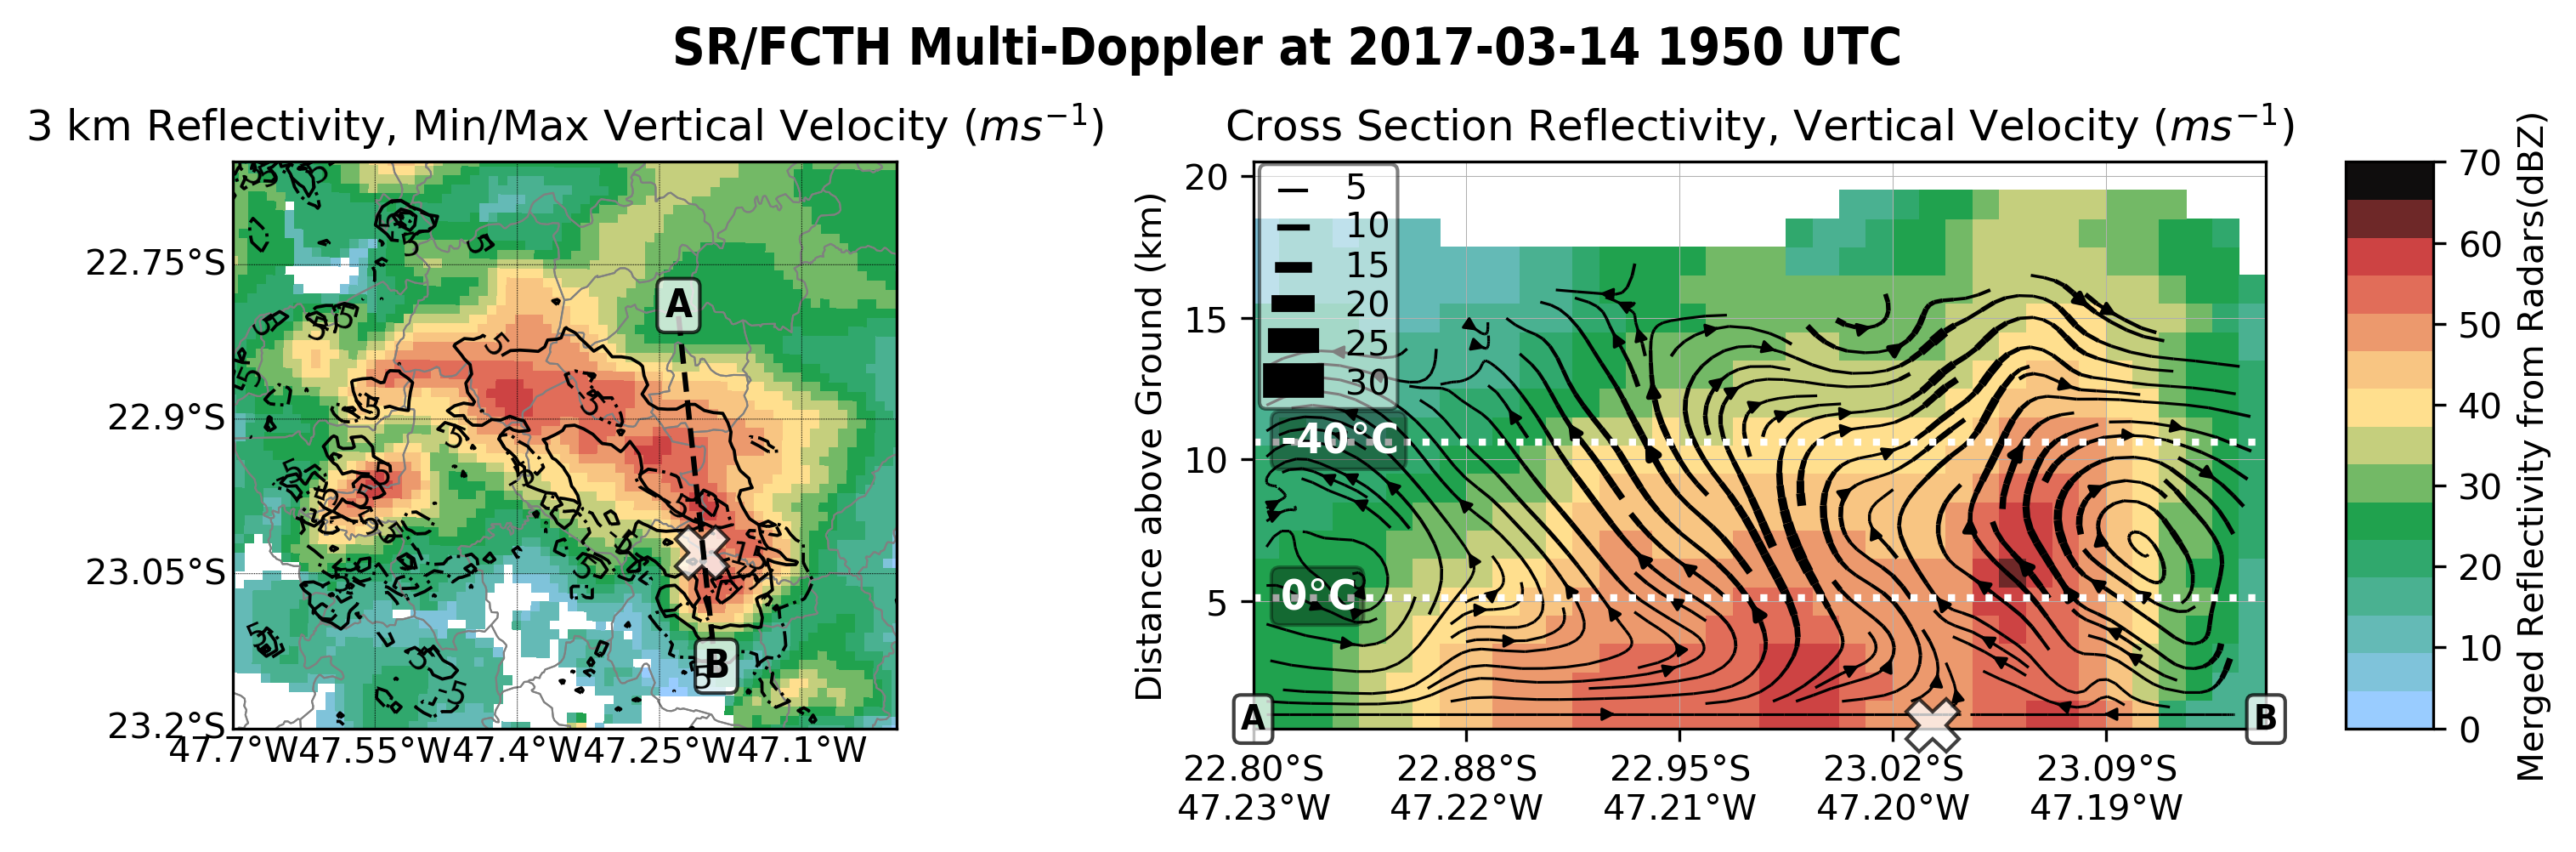
\includegraphics[width=\columnwidth]{../MultiDoppler_Processing/figures/SR-FCTH 2017-03-14 1950 UTC.png}
	\label{dopplera_20170314_2} \\
	\vspace{-15pt}
	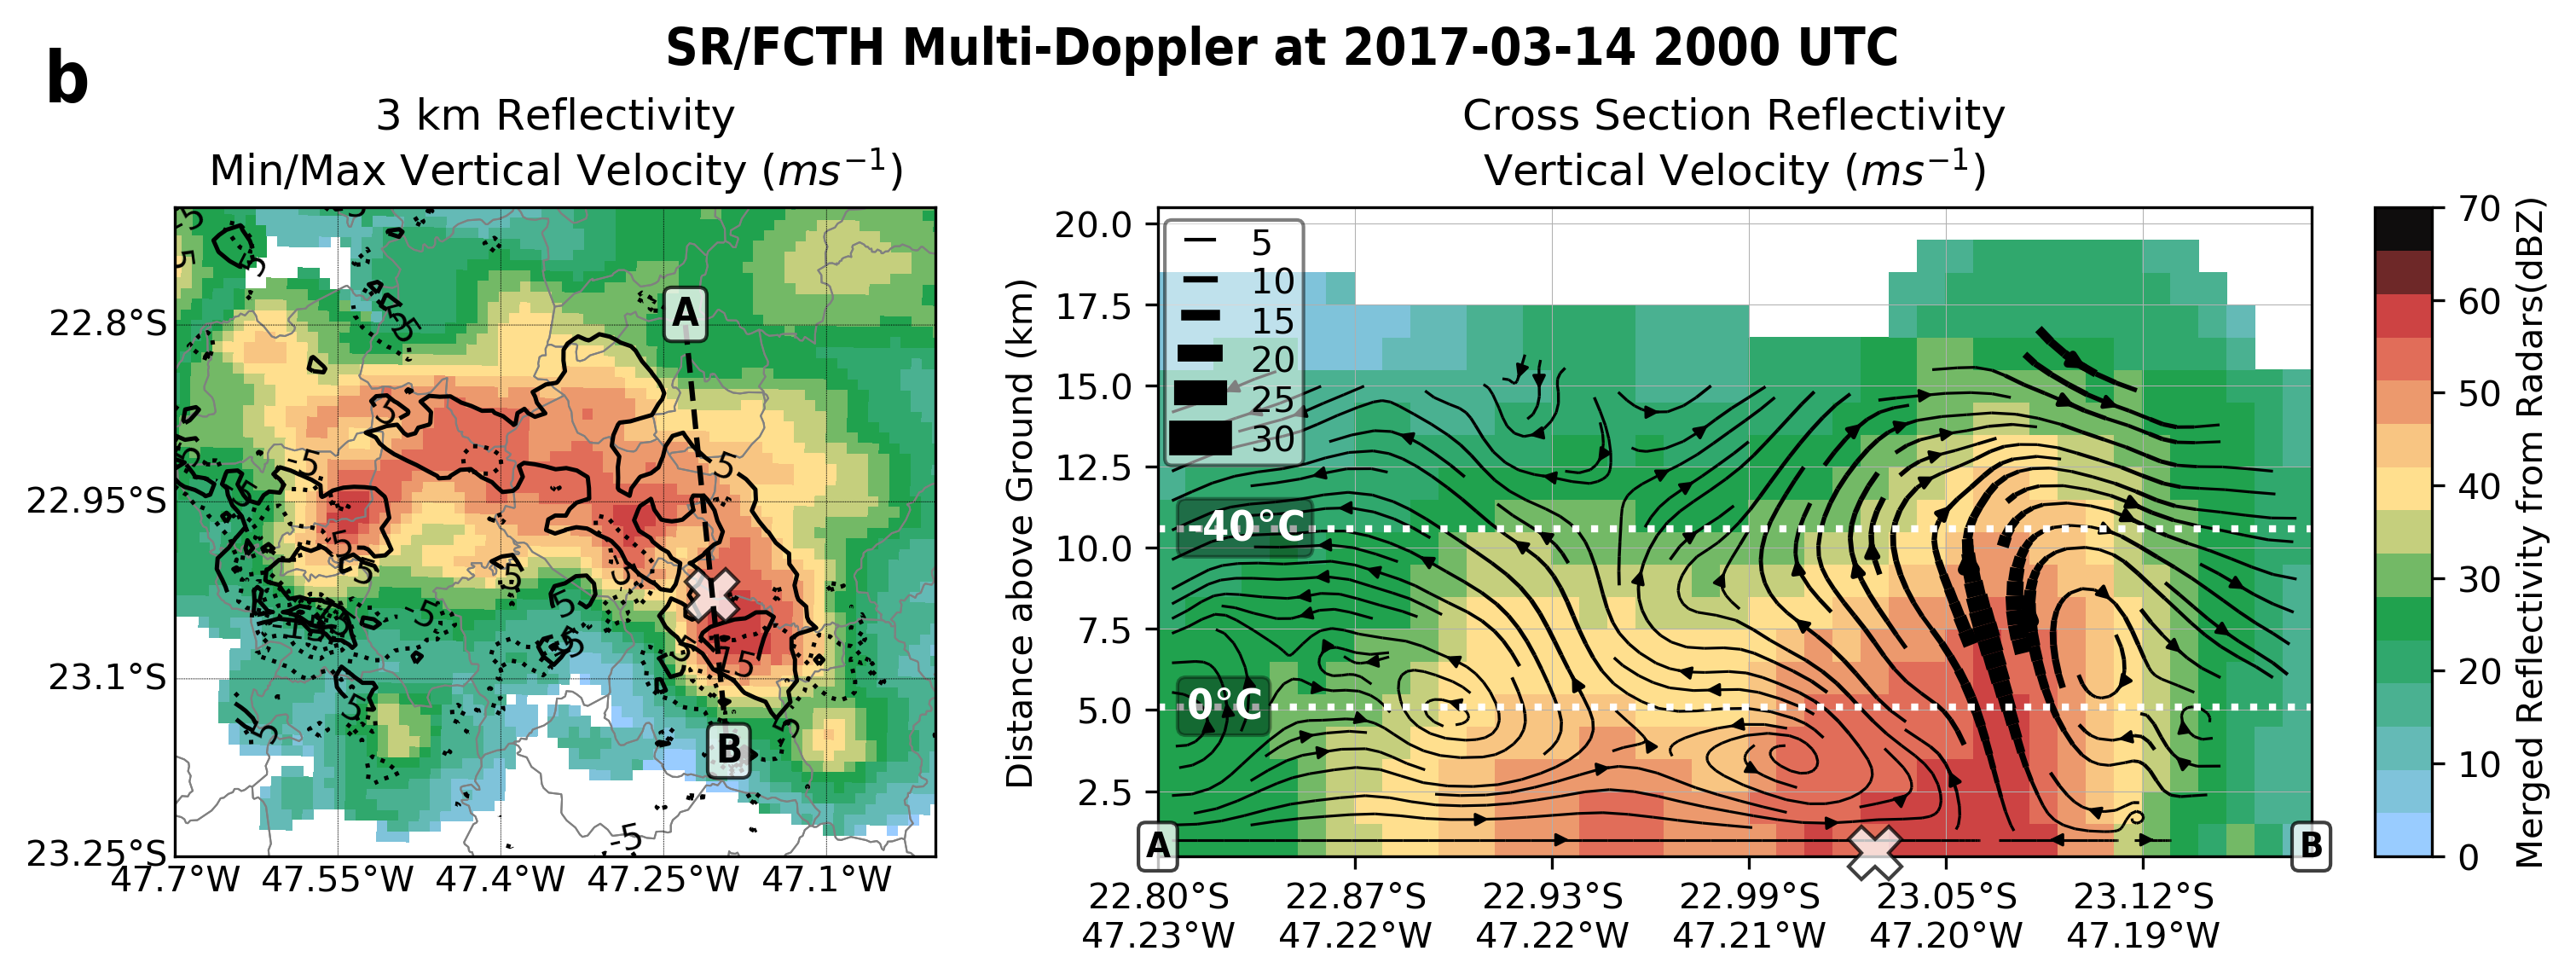
\includegraphics[width=\columnwidth]{../MultiDoppler_Processing/figures/SR-FCTH 2017-03-14 2000 UTC.png}
	\label{dopplerb_20170314_2} \\
	\vspace{-5pt}
	\legend{Fonte: Produzido pela autora.}
\end{figure}

\subsection{2017-11-15}

\subsubsection{Ambiente Sinótico}\label{sinotica_20171115}

\begin{figure}[htb]
	\begin{center}
		\caption{Campos da reanálise do ERA5 em 2017-11-15: Pressão ao nível médio do mar, espessura entre $1000$ e $500\:hPa$ e velocidade do vento em $250\:hPa$ às 1200 (a) e 1800 UTC (c); altura geopotencial em $850\:hPa$, cisalhamento do vento entre $1000$ e $500\:hPa$ e CAPE em superfície às 1200 (b) e 1800 UTC (d)} 
		\label{era5_20171115_main}
		\subfloat[]{\includegraphics[width=0.5\columnwidth]{../Reanalysis_Processing/figures/ERA5_SA_sfc-jets_201711151200.png}
			\label{era5_2017111512_jets}}
		\subfloat[]{\includegraphics[width=0.5\columnwidth]{../Reanalysis_Processing/figures/ERA5_SA_cape-shear_2017111512.png}
			\label{era5_2017111512_cape}} \\
		\subfloat[]{\includegraphics[width=0.5\columnwidth]{../Reanalysis_Processing/figures/ERA5_SA_sfc-jets_201711151800.png}
			\label{era5_2017111518_jets}}
		\subfloat[]{\includegraphics[width=0.5\columnwidth]{../Reanalysis_Processing/figures/ERA5_SA_cape-shear_2017111518.png}
			\label{era5_2017111518_cape}} \\
		\legend{Fonte: Produzido pela autora.}
	\end{center}
\end{figure}

\begin{figure}[htb]
	\begin{center}
		\caption{Plotagem Skew-T Log-P da radiossondagem do Campo de Marte (SP) com hodógrafa do vento e índices CAPE e CIN em 2017-11-15 1200 UTC.} 
		\label{sondagem_20171115}
		%		\setcaptionmargin{1cm}
		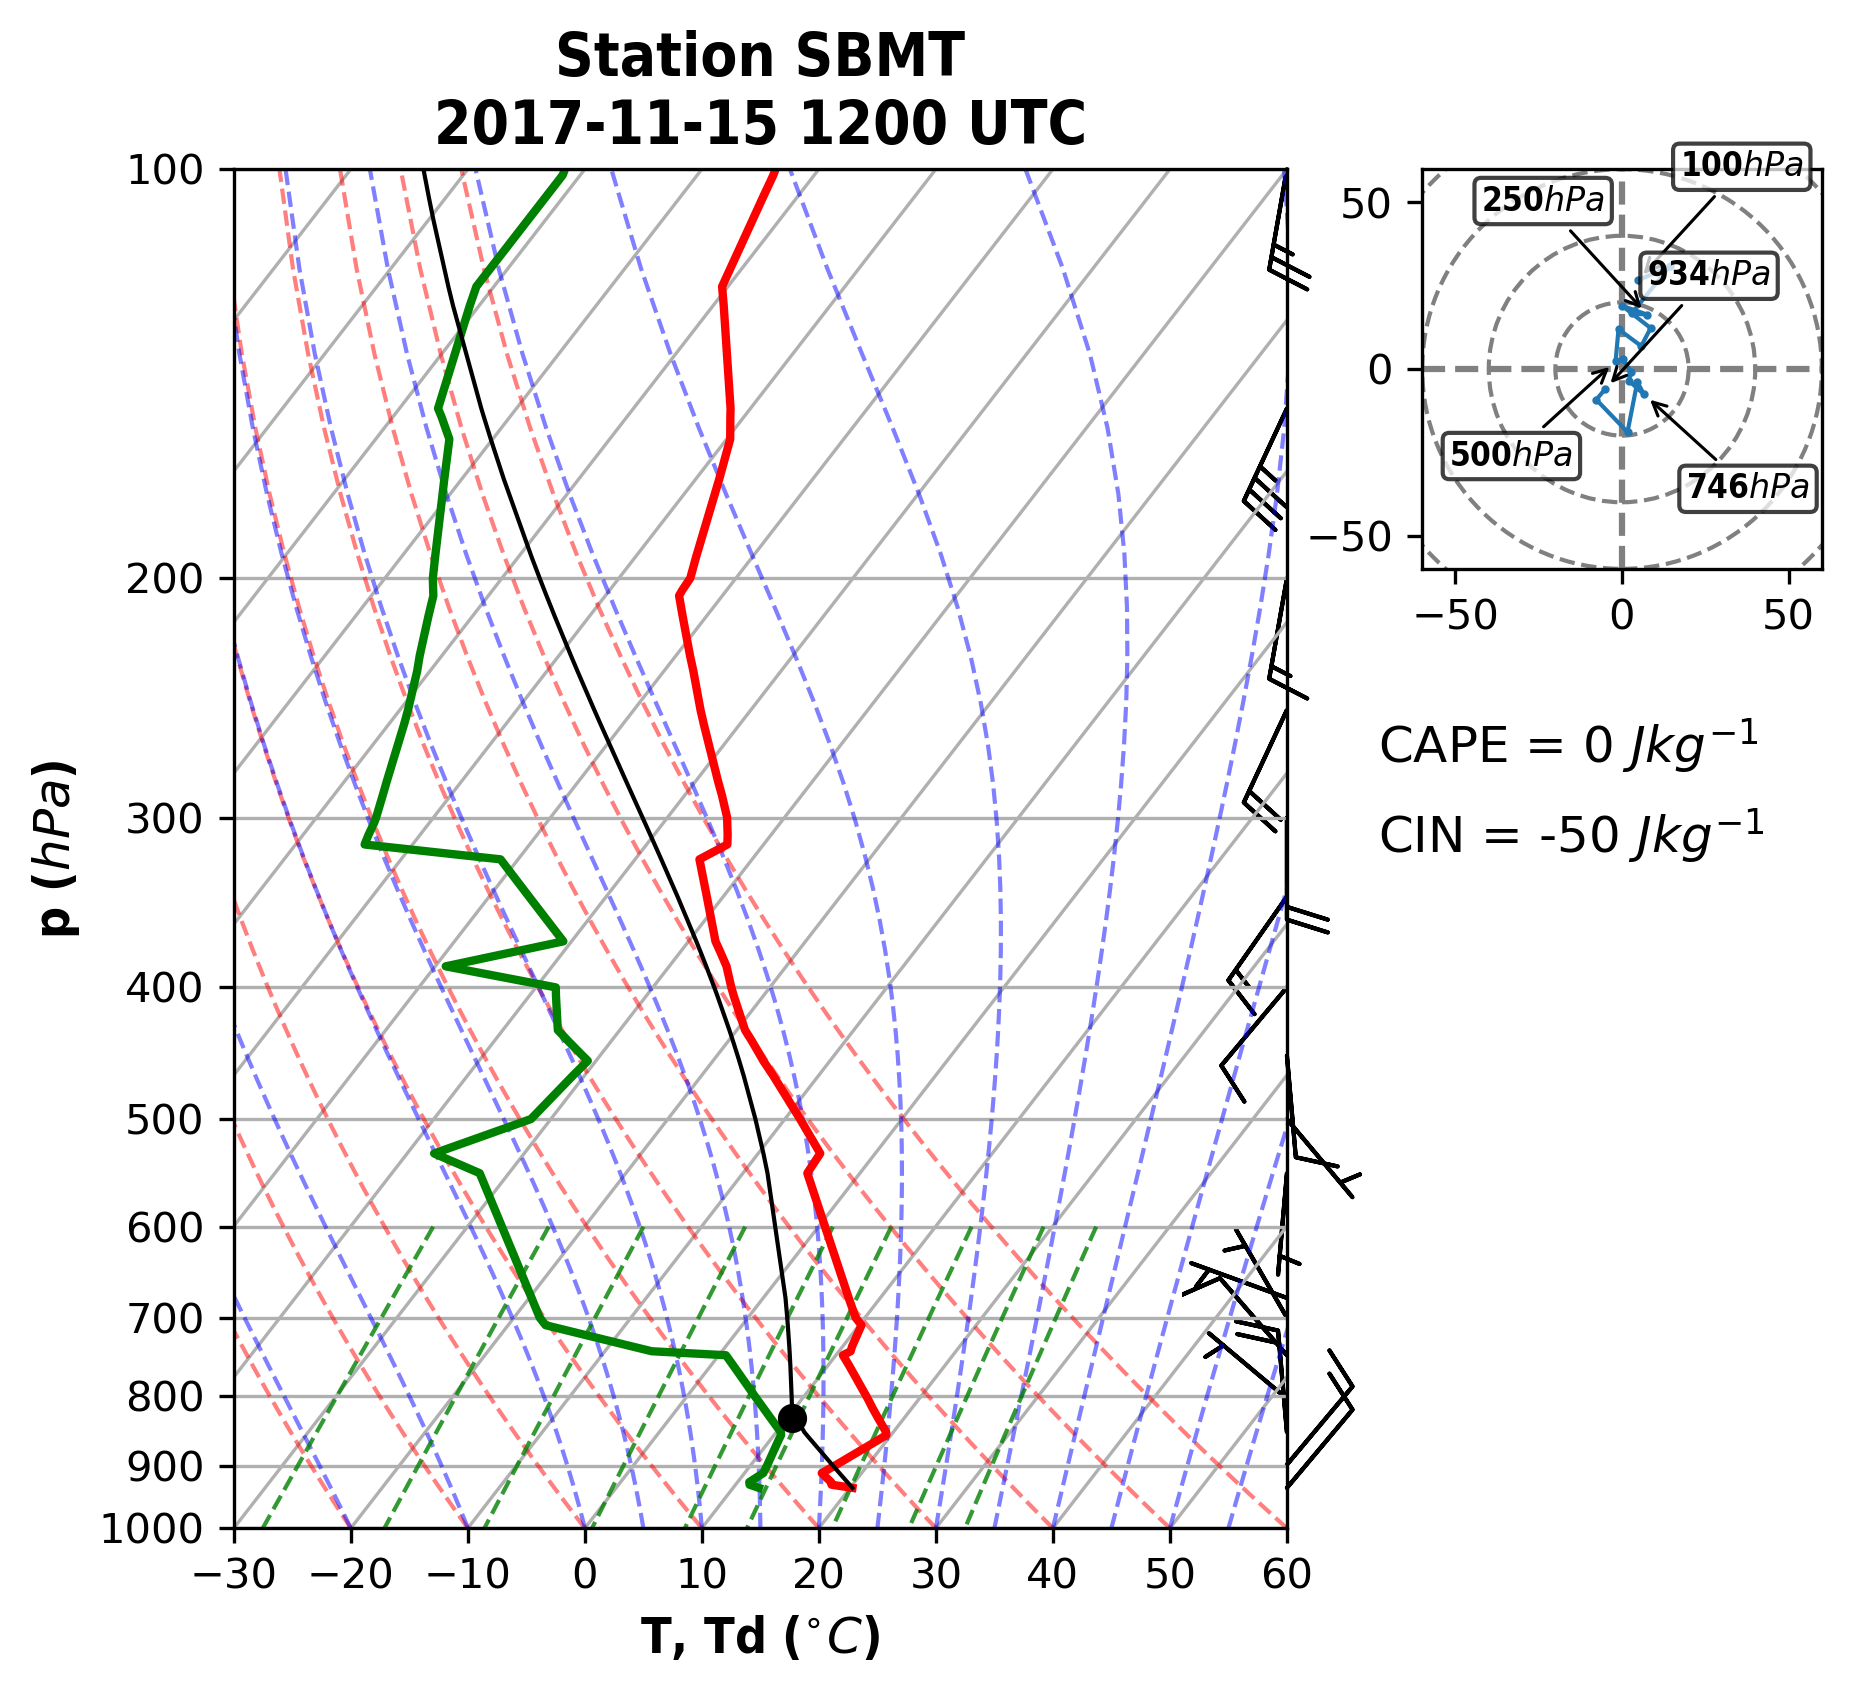
\includegraphics[width=0.9\columnwidth]{../Sounding_Processing/figures/sounding_SBMT2017111512UTC.png}
		\legend{Fonte: Produzido pela autora.}
	\end{center}
\end{figure}

\begin{figure}[htb]
	\begin{center}
		\caption{Imagem de satélite do canal 13 do GOES-16 mostrando a temperatura de brilho do topo das nuvens na América do Sul em 2017-11-15 1800 UTC.} 
		\label{goes16_sa_20171115}
		%		\setcaptionmargin{1cm}
		\includegraphics[width=0.75\columnwidth]{../Satellite_Processing/figures/Band_13/GOES16_B13_SA_SD201711151800.png}
		\legend{Fonte: Produzido pela autora.}
	\end{center}
\end{figure}


\begin{figure}[htb]
	\begin{center}
		\caption{Imagem de satélite do canal 13 do GOES-16 mostrando a temperatura de brilho do topo das nuvens no estado de São Paulo em 2017-11-15 2100 (a) e 2200 UTC (b).} 
		\label{goes16_sp_20171115}
		\subfloat[]{\includegraphics[width=0.75\columnwidth]{../Satellite_Processing/figures/Band_13/GOES16_B13_SP-BR_SD201711152100.png}
			\label{goes16_sp_20171115_1}} \\
		\subfloat[]{\includegraphics[width=0.75\columnwidth]{../Satellite_Processing/figures/Band_13/GOES16_B13_SP-BR_SD201711152200.png}
			\label{goes16_sp_20171115_2}} \\
		\legend{Fonte: Produzido pela autora.}
	\end{center}
\end{figure}

\subsubsection{Eletrificação}\label{elec_20171115}

\begin{figure}[htb]
	\begin{center}
		\caption{Rastreamento (a) e localização dos flashes IC e CG (b) do sistema convectivo responsável pela queda de granizo em Indaiatuba em 2017-11-15. Os triângulos pretos indicam a localização dos hailpads.} 
		\label{track_flashes_20171115}
		%		\setcaptionmargin{1cm}
		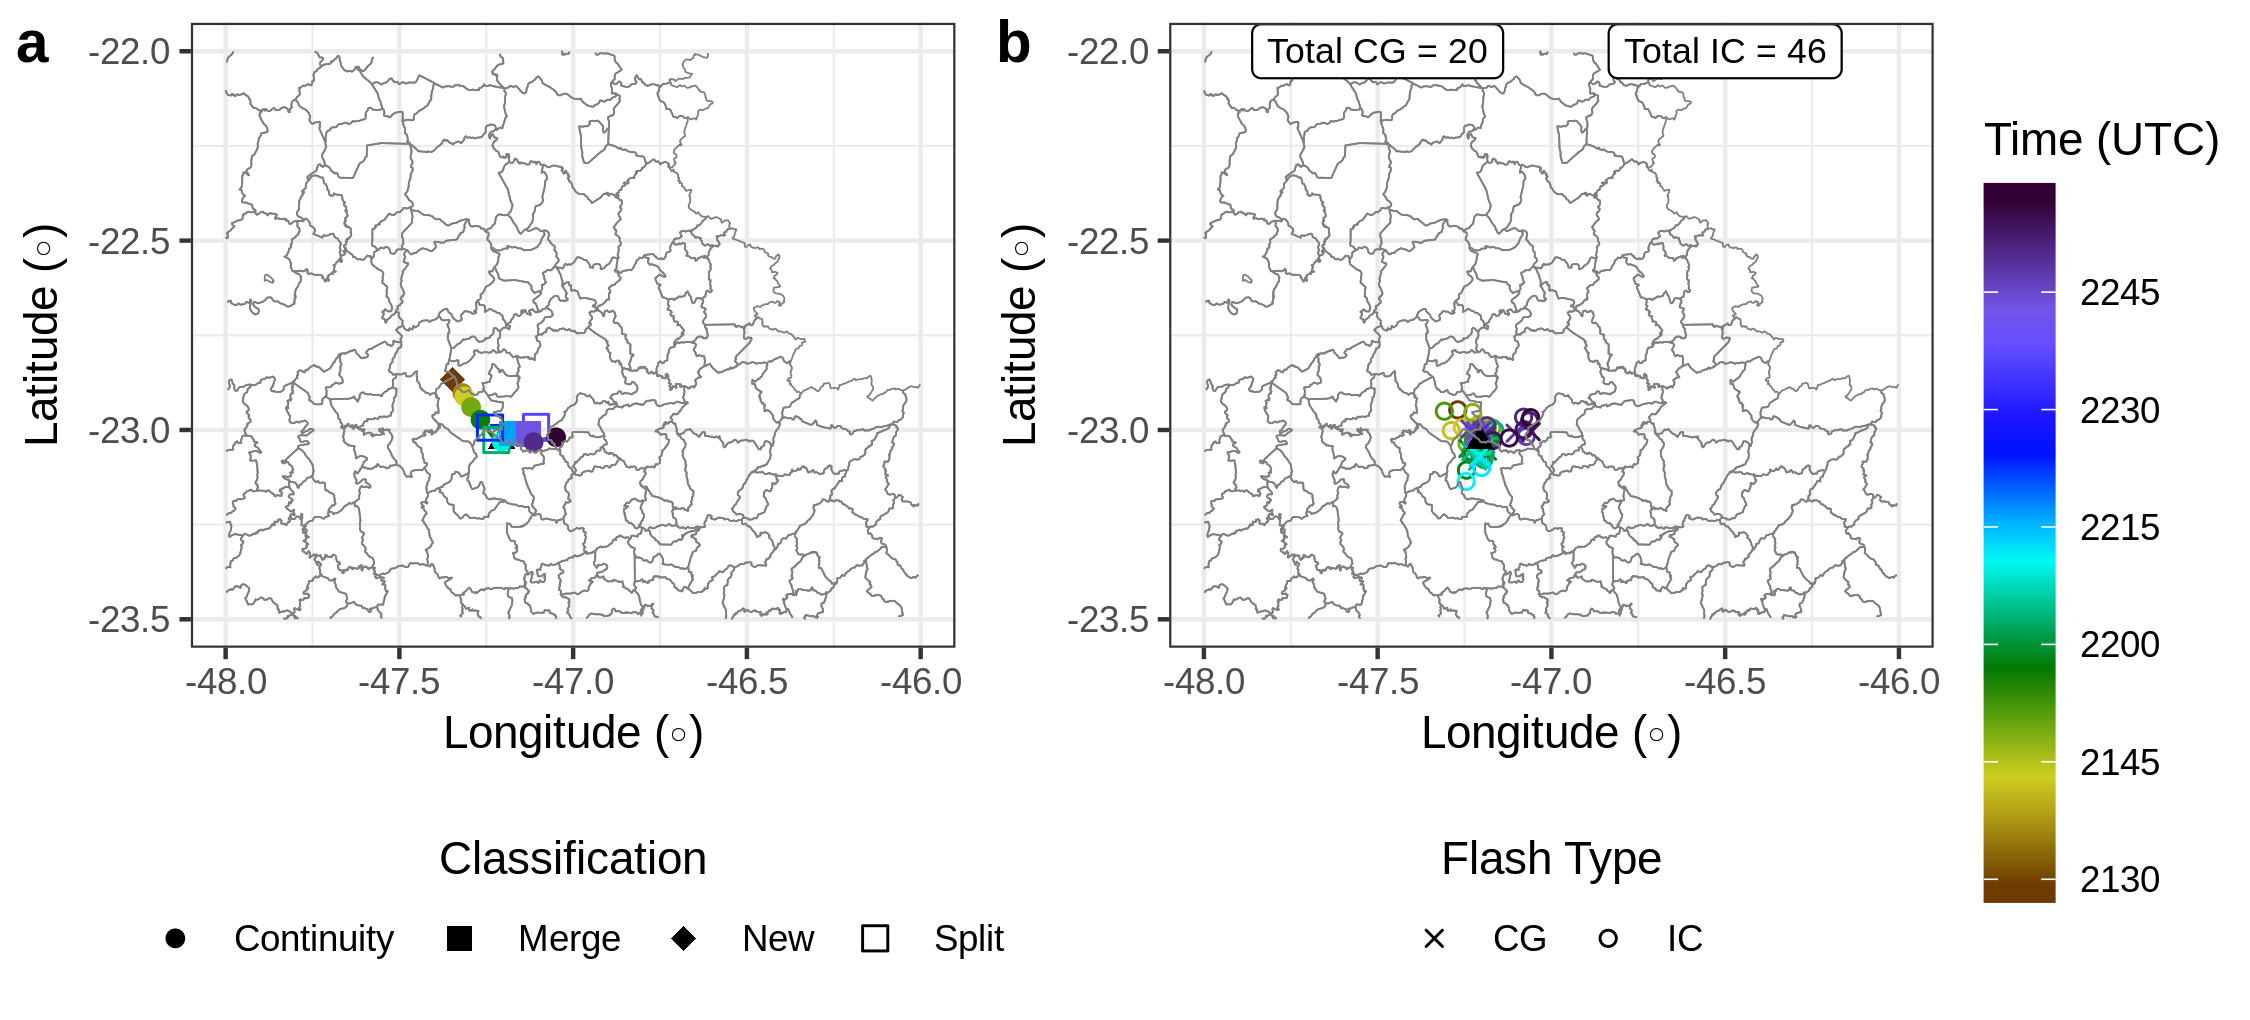
\includegraphics[width=\columnwidth]{../General_Processing/figures/track_flashes_20171115.png}
		\legend{Fonte: Produzido pela autora.}
	\end{center}
\end{figure}

\subsubsection{Microfísica}\label{micro_20171115}

\begin{figure}[hp]
	\centering
	\caption{Corte horizontal em $3\:km$ de altura e vertical entre os pontos A e B de campos do radar da FCTH em 2017-11-15 2150 UTC, quando houve queda de granizo em Indaiatuba: Refletividade corrigida (a) e diferencial (b), fase diferencial específica (c) e coeficiente de correlação (d). O 'x' indica a localização do hailpad e as isotermas de $0$ e $-40^{\circ}C$ foram definidas a partir da radiossondagem de SMBT}
	\label{radar_20171115}
	\vspace{-5pt}
	\includegraphics[width=\columnwidth]{../Radar_Processing/figures/ppis/classification/FCTH Corrected Reflectivity 2017-11-15 2150 UTC.png}
	\label{z_20171115} \\
	\vspace{-15pt}
	\includegraphics[width=\columnwidth]{../Radar_Processing/figures/ppis/classification/FCTH Differential Reflectivity 2017-11-15 2150 UTC.png}
	\label{zdr_20171115} \\
	\vspace{-15pt}
	\includegraphics[width=\columnwidth]{../Radar_Processing/figures/ppis/classification/FCTH Specific Differential Phase 2017-11-15 2150 UTC.png}
	\label{kdp_20171115} \\
	\vspace{-15pt}
	\includegraphics[width=\columnwidth]{../Radar_Processing/figures/ppis/classification/FCTH Cross Correlation Ratio 2017-11-15 2150 UTC.png}
	\label{rho_20171115} \\
	\vspace{-5pt}
	\legend{Fonte: Produzido pela autora.}
\end{figure}

\begin{figure}[htb]
	\centering
	\caption{Corte horizontal em $3\:km$ de altura e vertical entre os pontos A e B de campos derivados do radar da FCTH em 2017-11-15 2150 UTC, quando houve queda de granizo em Indaiatuba: Identificação de hidrometeoros (a) e massas de água líquida (b) e gelo (c). O 'x' indica a localização do hailpad e as isotermas de $0$ e $-40^{\circ}C$ foram definidas a partir da radiossondagem de SMBT} 
	\label{radar_derived_20171115}
	\vspace{-5pt}
	\includegraphics[width=\columnwidth]{../Radar_Processing/figures/ppis/classification/FCTH Hydrometeor ID 2017-11-15 2150 UTC.png}
	\label{hid_20171115} \\
	\vspace{-15pt}
	\includegraphics[width=\columnwidth]{../Radar_Processing/figures/ppis/classification/FCTH Liquid Water Mass 2017-11-15 2150 UTC.png}
	\label{ml_20171115} \\
	\vspace{-15pt}
	\includegraphics[width=\columnwidth]{../Radar_Processing/figures/ppis/classification/FCTH Ice Water Mass 2017-11-15 2150 UTC.png}
	\label{mi_20171115} \\
	\vspace{-5pt}
	\legend{Fonte: Produzido pela autora.}
\end{figure}

\subsubsection{Cinemática}\label{cinematica_20171115}

\begin{figure}[htb]
	\centering
	\caption{Corte horizontal em $3\:km$ de altura e vertical entre os pontos A e B de refletividade e velocidade do vento (correntes ascendentes e descendentes máximas no painel da esquerda, escoamento no painel da direita) derivado por Multi-Doppler em 2017-11-15 às 2140 (a) e 2150 UTC (b), quando houve queda de granizo em Cosmópolis. O 'x' indica a localização do hailpad e as isotermas de $0$ e $-40^{\circ}C$ foram definidas a partir da radiossondagem de SMBT} 
	\label{doppler_20171115}
	\vspace{-5pt}
	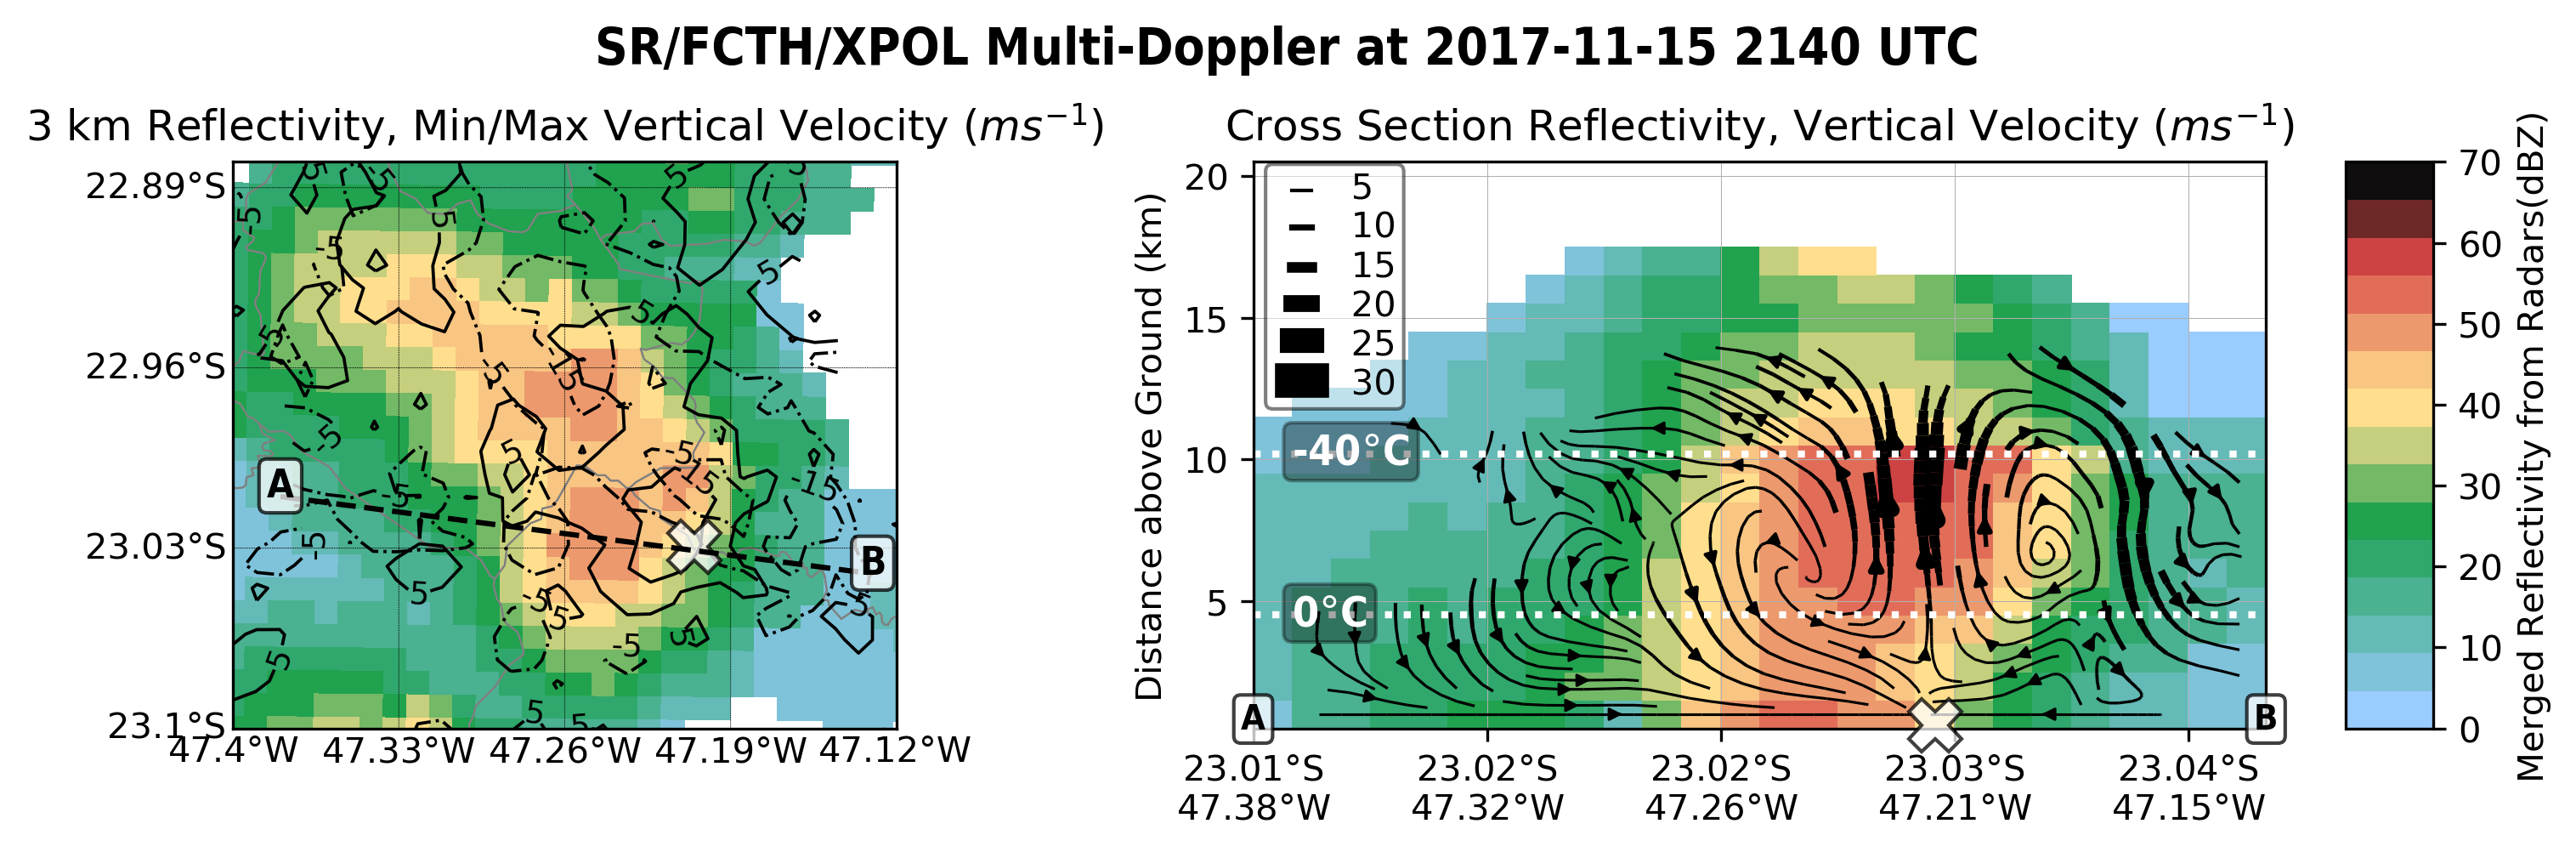
\includegraphics[width=\columnwidth]{../MultiDoppler_Processing/figures/SR-FCTH-XPOL 2017-11-15 2140 UTC.png}
	\label{dopplera_20171115} \\
	\vspace{-15pt}
	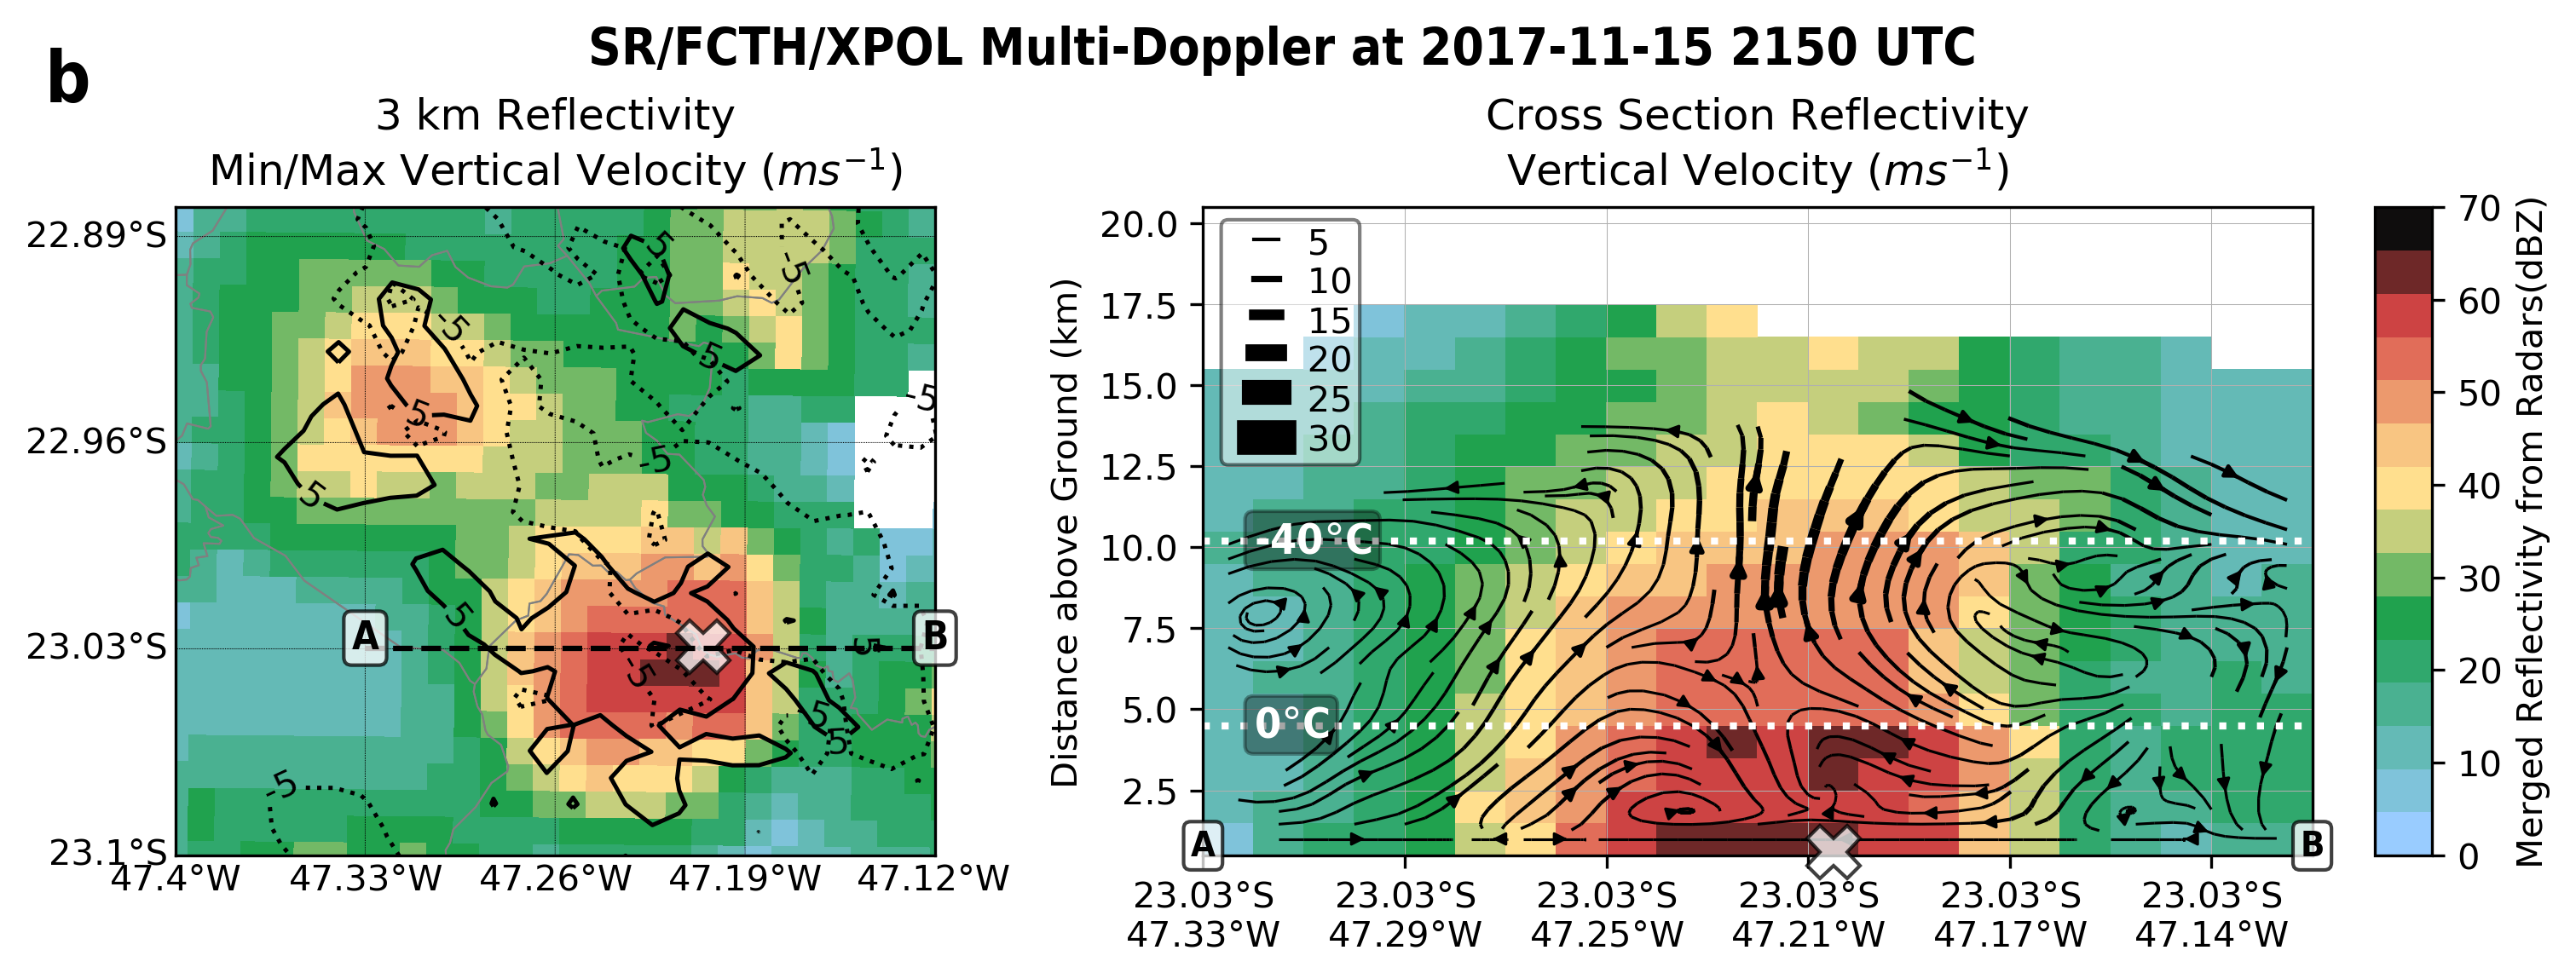
\includegraphics[width=\columnwidth]{../MultiDoppler_Processing/figures/SR-FCTH-XPOL 2017-11-15 2150 UTC.png}
	\label{dopplerb_20171115} \\
	\vspace{-5pt}
	\legend{Fonte: Produzido pela autora.}
\end{figure}
